\documentclass[12pt,a4paper]{report}
\usepackage{dissertation}

\usepackage{tabularx}
\usepackage{tikz}

\usetikzlibrary{matrix,positioning,arrows.meta,fit,shadows.blur}


\makeglossaries
\makeindex


\logo{EE}{Escola de Engenharia}{}
\logoB{EE}{Escola de Engenharia}{}



\author{Rui Pedro Chaves Silva Lousada Alves}

\titleA{Monitorização de uma Arquitetura\\ de Microsserviços}
% \titleB{Título Título Título Título Título}
% \titleC{Título Título Título Título}

\masters{Mestrado em Engenharia Informática}
%\area{Área de especialização}
\supervisor{Professor Orlando Manuel Oliveira Belo}
\cosupervisor{Ricardo Rodrigues}

\bibpunct[,]{(}{)}{;}{a}{,}{,}
\begin{document}
\setlength{\parindent}{0em}

%-- Covers
\input{covers/Covers}

%-- Document setup
\newgeometry{right=25mm, left=25mm, top=25mm, bottom=25mm}
\pagenumbering{roman}

\setlength{\parskip}{0pt}
\setlength{\parindent}{1.5em}

%-- Preamble
\input{preamble/Copyright}
\chapter*{Agradecimentos}
\setlength{\parskip}{1em}

% Em primeiro lugar, manifesto o meu sincero agradecimento ao meu orientador, Professor Orlando Belo pela orientação inestimável, conselhos esclarecedores e dedicação inabalável ao meu desenvolvimento académico. A sua experiência e incentivo foram determinantes em todas as fases do processo de investigação e redação, não sendo este trabalho possível sem o seu contributo.

% De igual modo, expresso o meu profundo reconhecimento ao DTx-Colab por me ter proporcionado a oportunidade de desenvolver esta investigação em ambiente empresarial, integrada no projeto R2UT. Esta colaboração permitiu-me obter uma perspetiva prática e aplicar o conhecimento adquirido em contexto real, aumentando significativamente o impacto e a relevância desta tese.

% O meu agradecimento sentido dirige-se igualmente à minha família, cujo apoio incondicional e sacrifícios foram fundamentais para atingir estas metas académicas e pessoais. Sou especialmente grato aos meus pais, Rui e Domingas. Expresso também a minha profunda gratidão à minha namorada, Leonor, pela paciência, compreensão e encorajamento prestados ao longo desta caminhada.

% Quero ainda expressar um agradecimento especial ao meu colega e amigo André, pelo tempo disponibilizado, pela partilha de conhecimento e pela ajuda prestada nos momentos de maior exigência técnica. A sua colaboração e disponibilidade foram essenciais para ultrapassar vários desafios durante o desenvolvimento deste trabalho.

% Por fim, agradeço a todos os meus verdadeiros amigos pela companhia, estímulo e presença constante nos momentos de maior desafio. O vosso apoio foi, sem dúvida, uma parte fundamental desta jornada.

Em primeiro lugar, manifesto o meu sincero agradecimento ao meu orientador, Professor Orlando Belo, pela orientação inestimável, conselhos esclarecedores e dedicação inabalável ao meu desenvolvimento académico. A sua experiência e incentivo foram determinantes em todas as fases do processo de investigação e redação, não sendo este trabalho possível sem o seu contributo.

De igual modo, expresso o meu profundo reconhecimento ao meu coorientador Ricardo Rodrigues, pelo acompanhamento próximo, orientação técnica e valiosos contributos ao longo deste trabalho. O seu apoio e disponibilidade foram essenciais para o desenvolvimento desta investigação e para o meu crescimento científico e profissional.

Expresso também o meu reconhecimento ao DTx-Colab por me ter proporcionado a oportunidade de desenvolver esta investigação em ambiente empresarial, integrada no projeto R2UT. Esta colaboração permitiu-me obter uma perspetiva prática e aplicar o conhecimento adquirido em contexto real, aumentando significativamente o impacto e a relevância desta tese.

O meu agradecimento sentido dirige-se igualmente à minha família, cujo apoio incondicional e sacrifícios foram fundamentais para atingir estas metas académicas e pessoais. Sou especialmente grato aos meus pais, Rui e Domingas. Expresso também a minha profunda gratidão à minha namorada, Leonor, pela paciência, compreensão e encorajamento prestados ao longo desta caminhada.

Quero ainda expressar um agradecimento especial ao meu colega e amigo André, pelo tempo disponibilizado, pela partilha de conhecimento e pela ajuda prestada nos momentos de maior exigência técnica. A sua colaboração e disponibilidade foram essenciais para ultrapassar vários desafios durante o desenvolvimento deste trabalho.

Por fim, agradeço a todos os meus verdadeiros amigos pela companhia, estímulo e presença constante nos momentos de maior desafio. O vosso apoio foi uma parte fundamental desta jornada.

\setlength{\parskip}{0em}
\input{preamble/StatementofIntegrity}
\chapter*{Resumo}

As arquiteturas de microsserviços permitem construir sistemas flexíveis, escaláveis e modulares em ambientes distribuídos. Contudo, a sua natureza dinâmica aumenta a complexidade dos processos de monitorização contínua, deteção de falhas e resposta proativa a eventos críticos.
Neste trabalho de dissertação, foi implementada uma plataforma para a monitorização e gestão de alertas de infraestruturas baseadas em microsserviços, com aplicação prática na indústria da construção modular. A solução desenvolvida integra ferramentas \textit{open source} — \textit{Prometheus}, \textit{Grafana}, \textit{Loki} (como alternativa à \textit{ELK Stack}) e \textit{Jaeger} — suportadas pelo \textit{OpenTelemetry} para a recolha padronizada de métricas, \textit{logs} e rastreio (\textit{tracing}) distribuído.
Para além disso, foram definidos cenários de alerta e mecanismos de resposta automática, de forma a reforçar a resiliência e reduzir o tempo de indisponibilidade da infraestrutura em monitorização.
Os resultados obtidos demonstram ganhos significativos em visibilidade ponta-a-ponta e uma redução nos tempos médios de deteção e resolução de incidentes (\textit{MTTD} e \textit{MTTR}), comprovando a viabilidade de uma pilha de observabilidade aberta, escalável e alinhada com requisitos de produção.


\paragraph{Palavras-chave:} Arquitetura de Microsserviços, Contentorização, Kubernetes, Monitorização de Sistemas Distribuídos, Docker, Deteção e Resolução de Falhas.


\cleardoublepage

\chapter*{Abstract}

Microservices architectures enable the development of flexible, scalable, and modular systems in distributed environments. However, their dynamic nature increases the complexity of continuous monitoring, fault detection, and proactive response to critical events.
This dissertation presents the implementation of a monitoring and alert management platform for microservices-based infrastructures, with practical application in the modular construction industry. The proposed solution integrates \textit{open source} tools - \textit{Prometheus}, \textit{Grafana}, \textit{Loki} (as an alternative to the \textit{ELK Stack}), and \textit{Jaeger} - supported by \textit{OpenTelemetry} for standardized collection of metrics, \textit{logs}, and distributed \textit{tracing}.
Furthermore, alert scenarios and automated response mechanisms were defined to strengthen system resilience and reduce infrastructure downtime.
The results demonstrate significant gains in end-to-end visibility and a reduction in the mean time to detect and resolve incidents (\textit{MTTD} and \textit{MTTR}), validating the feasibility of an open, scalable, and production-ready observability stack.



\paragraph{Keywords} Microservices Architecture, Containerization, Kubernetes, Distributed Systems Monitoring, Docker, Fault Detection and Troubleshooting.

\cleardoublepage


\phantomsection
\tableofcontents

\cleardoublepage
\listoffigures

% List of tables
\listoftables
\clearpage

% Acronyms
\printglossary[type=\acronymtype,nonumberlist, title={Acrónimos}]

% Glossary
\printglossary[title={Glossário}, nonumberlist]

\cleardoublepage
\pagenumbering{arabic}

%-- Dissertation 
% \part{Material Introdutório}

\chapter{Introdução}

\section{Contextualização}

As arquiteturas de microsserviços têm emergido como uma das abordagens mais populares no desenvolvimento de software moderno, possibilitando a criação de sistemas escaláveis, modulares e fáceis de manter \cite{Larrucea2018}. No entanto, o caráter distribuído dessa arquitetura introduz desafios significativos na monitorização, \textit{logging} e alerta dos seus componentes, especialmente em ambientes dinâmicos e baseados em \textit{containers}, como os geridos com \textit{Docker} e \textit{Kubernetes} \cite{Liu2020}. A necessidade de uma monitorização eficaz torna-se ainda mais crítica em ambientes dinâmicos e baseados em \textit{containers}, nos quais costumam operar aplicações distribuídas, em grande escala, que estão sujeitas a variações constantes nas cargas de trabalho com que têm de lidar. A adoção de estratégias de monitorização é essencial para garantir a estabilidade e o desempenho, permitindo a identificação proativa de anomalias e a resolução eficiente de falhas.

Ferramentas como \textit{Prometheus}, \textit{Grafana}, \textit{ELK Stack} e \textit{Jaeger} são amplamente utilizadas em aplicações de recolha e análise de \textit{logs}, monitorização de métricas e \textit{tracing} distribuído, proporcionando maior visibilidade sobre o comportamento dos serviços em execução. No contexto de aplicações baseadas em microsserviços, em que a comunicação entre componentes é altamente distribuída, uma infraestrutura de monitorização desempenha um papel crucial na manutenção da confiabilidade e escalabilidade da plataforma. Assim, garantir a monitorização e o acompanhamento dos serviços e da aplicação desenvolvida permite não apenas detetar rapidamente problemas, mas também implementar respostas automatizadas a eventos críticos, reduzindo o tempo de inatividade e aumentando a eficiência operacional dos sistemas.



\section{Motivação}

O projeto \textit{R2UT (Ready to Use Technology)} teve como principal objetivo impulsionar a transformação digital da indústria da construção civil em Portugal, promovendo a adoção de modelos de construção modular, industrializada e tecnologicamente avançada. Desenvolvido através da colaboração entre empresas e centros de investigação, o projeto procurou criar soluções inovadoras capazes de aumentar a produtividade, reduzir o desperdício e acelerar o processo construtivo, assegurando elevados padrões de qualidade e sustentabilidade.

No âmbito desta iniciativa, foi desenvolvida uma plataforma digital integrada destinada a suportar as diferentes fases do ciclo de vida dos edifícios pré-fabricados, desde o planeamento e conceção até à operação e manutenção. Esta plataforma combinou tecnologias de automação, \textit{Internet of Things (IoT)} e gestão inteligente de dados, permitindo o acompanhamento em tempo real do desempenho dos sistemas e dispositivos distribuídos.

Contudo, a crescente complexidade da arquitetura da plataforma e o número elevado de serviços distribuídos introduziram novos desafios relacionados com a monitorização, deteção de falhas e gestão do desempenho. Problemas como falhas na comunicação entre serviços, anomalias de desempenho e limitações de escalabilidade podiam comprometer a fiabilidade da infraestrutura e a integridade dos dados captados pelos dispositivos conectados \cite{Barakat2017}.

Neste contexto, esta dissertação teve como foco o desenvolvimento de uma solução de monitorização e gestão de alertas para a plataforma \textit{R2UT}, com o objetivo de garantir observabilidade, estabilidade e eficiência operacional. A solução proposta foi concebida de forma robusta e escalável, permitindo a deteção rápida de falhas e a implementação de respostas automáticas a eventos críticos.

Para tal, foi desenvolvida uma plataforma de monitorização baseada numa arquitetura de microsserviços, responsável pela recolha, centralização e análise de \textit{logs}, métricas e \textit{tracing} distribuído, através da integração de ferramentas amplamente utilizadas no ecossistema de observabilidade. O sistema resultante proporciona maior visibilidade sobre o comportamento dos serviços e componentes da aplicação \textit{R2UT}, contribuindo para um ambiente seguro, resiliente e de fácil manutenção, em alinhamento com os objetivos do projeto.

\section{Objetivos}
Este trabalho visa desenvolver uma plataforma de monitorização e alarmística para o projeto R2UT, assegurando uma gestão centralizada e em tempo real de microsserviços através de componentes \textit{open source}. Além de permitir respostas automatizadas a cenários críticos, a plataforma incluirá um \textit{dashboard} interativo para análise e filtragem avançada dos dados de monitorização e \textit{logs}, promovendo escalabilidade e resiliência no ambiente modular.
Para este trabalho de dissertação foram estabelecidos os seguintes objetivos:

\begin{itemize}
    \item Desenvolver uma plataforma de monitorização e alarmística para o projeto R2UT, utilizando componentes \textit{open source} com licenças de utilização aberta (como MIT ou Apache 2.0), garantindo segurança, escalabilidade e eficiência \cite{Mayer2017}. 
    \item Garantir a monitorização dos microsserviços da infraestrutura, proporcionando uma visão unificada e em tempo real das operações.
    \item Estudar e implementar uma estrutura de centralização de \textit{logs} para recolher e consolidar \textit{logs} de todos os microsserviços, facilitando a supervisão do fluxo de dados e a identificação de anomalias \cite{Cinque2022}.
    \item Incluir funcionalidades de resposta automatizada para acionar ações específicas em cenários críticos, como o escalonamento automático (\textit{autoscaling}) de serviços ou a execução de correções automáticas. 
    \item Desenvolver um \textit{dashboard} intuitivo e interativo para visualização, análise e aplicação de filtros avançados nos dados de monitorização e \textit{logs}, permitindo uma análise precisa e personalizável. 
\end{itemize}

\break

\section{Trabalho Realizado}

Ao longo deste trabalho, foi concebida e implementada uma plataforma de monitorização e gestão de alertas para o projeto R2UT, com o propósito de reforçar a observabilidade e a capacidade de supervisão da sua infraestrutura de microsserviços. A solução foi desenvolvida com recurso a componentes \textit{open source} sob licenças de utilização aberta, como MIT ou Apache 2.0, garantindo elevados níveis de segurança, escalabilidade e eficiência \cite{Mayer2017}.

A plataforma proposta permitiu centralizar a monitorização dos microsserviços, oferecendo uma visão consolidada e em tempo real do estado operacional do sistema. Para suportar esta monitorização, foi estudada e implementada uma estrutura de centralização de \textit{logs}, responsável pela recolha, agregação e análise dos registos gerados pelos diferentes serviços. Esta abordagem possibilitou a supervisão contínua do fluxo de dados, bem como a deteção de anomalias e falhas na execução dos componentes distribuídos \cite{Cinque2022}.

Complementarmente, foram desenvolvidos \textit{dashboards} interativos e de fácil utilização, que permitem a visualização e análise detalhada das métricas, \textit{traces} e dos \textit{logs} recolhidos. Este painel oferece funcionalidades avançadas de filtragem e exploração de dados, facilitando a interpretação do comportamento dos serviços e suportando a tomada de decisões operacionais fundamentadas.

A solução implementada contribuiu de forma significativa para a melhoria da visibilidade e resiliência da plataforma R2UT, promovendo uma gestão mais eficiente e proativa dos serviços num ambiente modular, escalável e distribuído.

\break


\section{Estrutura do Documento}

Além deste capítulo introdutório, a presente dissertação encontra-se organizada da seguinte forma:

\begin{itemize}
    \item \textbf{Capítulo 2 – Arquiteturas de Microserviços} \\
    Este capítulo apresenta a evolução e os fundamentos das arquiteturas de microsserviços, explorando a sua emergência como paradigma moderno no desenvolvimento de sistemas distribuídos. São discutidos os princípios que regem este modelo arquitetónico, a sua comparação com arquiteturas monolíticas e orientadas a serviços, bem como os desafios técnicos e organizacionais associados. Por fim, aborda-se a adoção de microserviços em contextos de larga escala e em ambientes de computação em nuvem.

    \item \textbf{Capítulo 3 – Monitorização e Observabilidade em Microserviços} \\
    Este capítulo analisa a importância da monitorização em sistemas distribuídos e introduz o conceito de observabilidade, sustentado nos seus três pilares fundamentais: \textit{logs}, métricas e \textit{tracing}. São descritas as principais ferramentas e técnicas utilizadas neste domínio, nomeadamente Prometheus, Grafana, Loki/ELK, Jaeger e OpenTelemetry. Adicionalmente, discutem-se os desafios atuais e tendências emergentes, incluindo a integração de abordagens baseadas em Inteligência Artificial para Operações (\textit{AIOps}).

    \item \textbf{Capítulo 4 – Implementação da Solução de Observabilidade} \\
    Neste capítulo é apresentada a implementação prática da solução proposta, abordando os desafios inerentes à orquestração de \textit{containers} e à integração de ferramentas avançadas de monitorização. São explorados conceitos como \textit{tracing} distribuído, padrões de resiliência, definição de alertas e práticas de observabilidade, fundamentais para assegurar a estabilidade e eficiência de sistemas baseados em microsserviços.

    \item \textbf{Capítulo 5 – Visualização e Análise dos Dados} \\
    Este capítulo apresenta os mecanismos de visualização e análise de dados implementados para suportar a monitorização do sistema. São explorados os dashboards desenvolvidos no Grafana, evidenciando a forma como métricas, \textit{logs} e \textit{traces} são agregados e correlacionados para facilitar o diagnóstico de problemas e a avaliação do desempenho do sistema. Adicionalmente, demonstra-se o processo analítico seguido, desde a deteção de comportamentos anómalos até à identificação da causa-raiz, bem como a integração de alertas automáticos através do \textit{Prometheus AlertManager} com notificação em canais operacionais (\textit{Slack}). Este capítulo visa demonstrar a eficácia da solução proposta na operacionalização da observabilidade, destacando a sua utilidade prática na supervisão contínua de ambientes baseados em microsserviços.

    \item \textbf{Capítulo 6 – Conclusões e Trabalho Futuro} \\
    Este capítulo apresenta as conclusões do trabalho desenvolvido, refletindo sobre os resultados obtidos e os desafios enfrentados. São também discutidas as contribuições do estudo para o projeto R2UT e para o avanço do conhecimento na área da observabilidade de sistemas distribuídos, bem como as perspetivas de evolução e as linhas de trabalho futuro.
    
\end{itemize}

\chapter{Microsserviços}

Nos últimos anos, as arquiteturas de microsserviços tornaram-se uma das abordagens mais populares no desenvolvimento de sistemas de software escaláveis e resilientes. A transformação arquitetural que este tipo de abordagem provocou, impulsionou nas organizações uma crescente necessidade para inovar rapidamente, para que fossem capazes de atender a requisitos de escalabilidade global e responder com total agilidade às constantes mudanças do mercado no qual se inserem. A mudança tecnológica assentou na evolução de arquiteturas monolíticas para sistemas compostos por múltiplos serviços independentes. Uma evolução que reflete uma mudança organizacional como também cultural nas organizações. Neste capítulo abordamos o surgimento dos microsserviços, a sua evolução histórica e o seu posicionamento no contexto das arquiteturas de software atuais. Em particular, discutir-se-ão alguns dos desafios inerentes à sua adoção, os seus conceitos fundamentais e o percurso que levou à sua populariza-ção no domínio da Engenharia de Software.

\section{Emergência e Evolução}

\subsection{Limitações das Arquiteturas Monolíticas}

Antes da emergência dos microsserviços, a maioria das aplicações empresariais eram desenvolvidas seguindo uma arquitetura monolítica, na qual todos os componentes do sistema - interface de utilizador, lógica de negócio e acesso a dados - estão integrados num único bloco de código. Uma única “peça” de software. Embora esta abordagem simplifique o desenvolvimento inicial, à medida que a aplicação vai crescendo e evoluindo vão surgindo vários problemas devido a essa tão grande concentração de serviços num único sistema \cite{Villamizar2015}. A Figura \ref{fig:monolitica_microservicos} apresenta uma comparação estrutural entre uma arquitetura monolítica e uma arquitetura baseada em microsserviços. Entre os principais problemas identificados destacam-se:

\begin{itemize}
    \item Dificuldade de escalar equipas de desenvolvimento. Diferentes equipas precisam de trabalhar no mesmo código, o que provoca frequentemente conflitos e a necessidade de uma coordenação intensiva.
    \item Ciclo de \textit{deployment} prolongados. A necessidade de testar e distribuir toda a aplicação torna os processos de atualização complexos e arriscados;
    \item Falta de resiliência. A ocorrência de uma falha, num único componente, pode com-prometer toda a aplicação, o que pode gerar uma interrupção generalizada dos serviços do sistema.
\end{itemize}

Estas limitações tornaram-se ainda mais evidentes com o avanço da computação em nuvem e a exigência por uma disponibilização contínua de serviços.

A Figura \ref{fig:monolitica_microservicos} evidencia estas diferenças, mostrando como, numa arquitetura monolítica, todos os módulos se encontram num único artefacto, enquanto na arquitetura de microsserviços cada componente opera de forma independente, comunicando através de um API Gateway e podendo utilizar bases de dados próprias.


\begin{figure}[h]
    \centering
    \includegraphics[width=0.6\textwidth]{images/Diagramas/monilitica_vs_microservicos.png}
    \caption{Comparação entre arquitetura monolítica e arquitetura de microsserviços}
    \label{fig:monolitica_microservicos}
\end{figure}

\subsection{De SOA a microsserviços}


O conceito de decompor aplicações monolíticas em serviços autónomos não é novo. As Arquiteturas Orientadas a Serviços (SOA) surgiram no final dos anos 1990 e início dos anos 2000, como uma primeira forma de abordar os problemas impostos pelas arquiteturas monolíticas. Numa arquitetura deste tipo, as aplicações são organizadas como uma coleção de serviços que interagem por meio de um “barramento” de mensagens - \textit{Enterprise Service Bus} (ESB). Um ESB é um sistema de \textit{middleware} que permite a comunicação entre serviços distintos numa SOA. O ESB atua como um único intermediário central que gere toda a integração, faz o encaminhamento de mensagens, a transformação de dados e aplica as políticas de segurança definidas para os vários serviços do sistema. Embora um ESB simplifique a integração inicial, a sua centralização cria dependências e um potencial ponto de falha do sistema. Fragilidades como estas, fizeram com que se procurassem alternativas mais descentralizadas, como as arquiteturas baseadas em microsserviços \cite{Aziz2020}.

Embora as SOA tenham introduzido avanços significativos na modularização de sis-temas, também criaram alguns desafios consideráveis, nomeadamente:


\begin{itemize}
    \item Complexidade excessiva. A utilização de ESB centralizados introduziu um ponto único de falha e complexidade operacional;
    \item Rigidez nos contratos de serviços. A realização de alterações nos serviços do sistema exigiam mudanças pesadas no barramento e nos consumidores.
    \item Foco excessivo em tecnologias pesadas. Os padrões SOAP e WS-*, por exemplo, tornaram as integrações difíceis e pouco ágeis.
\end{itemize}

A arquitetura de microsserviços pode ser vista como uma evolução pragmática das SOA, mas focada na simplicidade, na independência e na automação de operações. Numa arquitetura de microsserviços, o barramento central é eliminado. Cada serviço comunica diretamente com os outros serviços, o que permite eliminar muitas das complexidades associadas aos tradicionais sistemas orientados a serviços.

A Figura \ref{fig:soa_microservicos} ilustra estas diferenças, evidenciando a centralização do ESB nas arquiteturas SOA em contraste com a comunicação distribuída e independente entre microsserviços.


\begin{figure}[h]
    \centering
    \includegraphics[width=0.6\textwidth]{images/Diagramas/soa_vs_microservicos.png}
    \caption{Comparação entre arquitetura SOA e arquitetura de microsserviços}
    \label{fig:soa_microservicos}
\end{figure}

\subsection{Fatores Tecnológicos e Organizacionais}

O surgimento dos microsserviços não pode ser atribuído apenas a fatores técnicos. Os fatores organizacionais também desempenharam um papel crucial nesse processo. Três dos movimentos principais que impulsionaram esta evolução foram \cite{Newman2015}:

\begin{itemize}
    \item \textbf{Computação em Nuvem.} A elasticidade da nuvem permitiu que aplicações fossem dimensionadas dinamicamente, o que incentivou arquiteturas a tirar partido dessa flexibilidade. Os microsserviços encaixam naturalmente nesse modelo, permitindo escalar apenas os componentes necessários.
    \item \textbf{\textit{DevOps} e \textit{Deployment} Contínuo.} A cultura \textit{DevOps} enfatizou a necessidade de integrar desenvolvimento e operações, automatizar pipelines de entrega contínua e reduzir ciclos de feedback. Os microsserviços permitem ciclos de desenvolvimento independentes para cada serviço, o que os permite alinhar com esses princípios.
    \item \textbf{\textit{Containers} e gestão de \textit{containers} } Tecnologias como \textit{Docker} ou \textit{Kubernetes} simplificaram significativamente a criação, o \textit{deploy} e a gestão de serviços independentes, tornando viável, em larga escala, o modelo dos microsserviços.
\end{itemize}

Segundo \cite{Lewis2014}, a capacidade de alinhar arquitetura de software com estruturas organizacionais ágeis, inspiradas na "Lei de Conway", foi um dos principais catalisadores para a adoção dos microsserviços. A “Lei de Conway”, formulada por Melvin Conway em 1968, estabelece que "any organization that designs a system (defined broadly) will produce a design whose structure is a copy of the organization's communication structure" \cite{Bailey2013} ("qualquer organização que projeta um sistema (em sentido amplo) inevitavelmente produzirá um design cuja estrutura é uma cópia da estrutura de comunicação da organização"). Essa observação implica que as estruturas organizacionais moldam, de maneira direta ou indireta, a arquitetura dos sistemas que desenvolvem.



\subsection{Popularização dos Microsserviços}

O termo microservices começou a ganhar popularidade em conferências técnicas por volta de 2011-2012, sendo posteriormente popularizado pelos trabalhos de autores como James Lewis, Martin Fowler e Sam Newman \cite{Lewis2014,Newman2015}. Empresas pioneiras como Netflix, Amazon, e Uber demonstraram publicamente os benefícios de arquiteturas baseadas em microsserviços, mostrando que era possível construir sistemas resilientes, escaláveis e altamente disponíveis a partir da composição de múltiplos serviços pequenos e independentes.
A experiência e dimensão dessas empresas inspirou uma grande adoção no setor, suportada por uma nova geração de ferramentas de monitorização e gestão distribuída, plataformas de infraestrutura como serviço (IaaS) e metodologias ágeis de desenvolvimento.
Atualmente, os microsserviços são amplamente reconhecidos como uma escolha estratégica para sistemas que exigem alta escalabilidade, independência organizacional e ciclos de entrega rápidos 
\cite{Dragoni2017}. No entanto, essa popularidade não elimina a complexidade técnica e organizacional que a arquitetura de microsserviços impõe, tema que será aprofundado nas próximas secções.


\section{O que são microsserviços?}

Após as limitações evidenciadas pelas arquiteturas monolíticas e a emergência de novos paradigmas tecnológicos e organizacionais, os microsserviços consolidaram-se como uma abordagem inovadora para o desenvolvimento de sistemas distribuídos modernos.

Nesta secção caracteriza-se a arquitetura de microsserviços, destacando as suas principais propriedades no cenário atual de engenharia de software.

\subsection{Definição Formal}

Um microsserviço é uma unidade modular de software criada com o intuito de executar uma funcionalidade especifica integrada num sistema maior. Os microsserviços são in-dependentes e autónomos, podendo assim serem desenvolvidos, testados e escalados separadamente de qualquer outro componente do sistema \cite{Jamshidi2018}. A principal característica dos microsserviços é a separação de responsabilidades. Cada ser-viço tem o seu propósito no contexto do sistema geral e, por isso, deve executar apenas o seu código, focando-se num único problema, aquilo que realmente lhe compete \cite{Newman2015}. Estes serviços são flexíveis e altamente escaláveis. Além disso permitem a utilização de tecnologias distintas na sua implementação; bem como o desenvolvimento paralelo de serviços e dimensionamneto granular por serviço (isto é, a capacidade de escalar apenas os serviços que efetivamente necessitam de mais recursos) \cite{Lewis2014}. Mais do que o tamanho do código, o termo "micro" enfatiza a responsabilidade limitada de cada serviço e a independência operacional, permitindo que estes sejam desenvolvidos, implementados e escalados de maneira isolada. Segundo \cite{Dragoni2017} o conceito de microsserviços surgiu como um refinamento de princípios preexistentes, como modularidade, separação de responsabilidades e princípios do desenvolvimento das SOA, mas com ênfase na autonomia e no alinhamento com domínios de negócio.


\subsection{Princípios e Principais Características}

Podemos caracterizar uma arquitetura de microserviços como tendo as seguintes características:

\begin{itemize}
    \item \textbf{Autonomia de desenvolvimento e \textit{deployment}.} Cada microserviço pode ser desenvolvido, testado, implementado e mantido de forma independente \cite{Newman2015}.
    
    \item \textbf{Especialização funcional.} Os serviços são organizados em torno de capacidades de negócio específicas, refletindo o princípio de responsabilidade única \cite{Newman2015}.
    
    \item \textbf{Comunicação leve.} Os microserviços utilizam protocolos de comunicação simples, como REST sobre HTTP, gRPC ou filas de mensagens assíncronas \cite{Dragoni2017}.
    
    \item \textbf{Independência tecnológica.} Os serviços podem ser implementados em diferentes linguagens de programação ou \textit{frameworks}, promovendo poliglotismo arquitetural 
    \cite{Richardson2018}.
    
    \item \textbf{Escalabilidade granular.} Serviços com maior procura podem ser escalados individualmente, permitindo alocação eficiente de recursos \cite{Lewis2014}.
    
    \item \textbf{Observabilidade.} Cada serviço é projetado para expor métricas, logs e \textit{tracing} distribuído, possibilitando monitorização e diagnóstico isolados \cite{Soldani2018}.
\end{itemize}


Este conjunto de princípios alinha a arquitetura de microserviços a práticas modernas de desenvolvimento ágil, DevOps e computação em nuvem.

\subsection{Componentes Típicos em Arquiteturas de microsserviços}

Geralmente, a implementação prática de microsserviços envolve diversos componentes arquiteturais adicionais, momeadamente:

\begin{itemize}
    \item \textbf{APIs Públicas.} Cada serviço expõe a sua funcionalidade por meio de uma interface bem definida, normalmente baseada em padrões como RESTful APIs ou gRPC.

    \item \textbf{As Base de Dados são Privadas.} Cada microsserviço é responsável pela sua própria persistência de dados, evitando assim dependências diretas entre serviços \cite{Dragoni2017}.

    \item \textbf{Mensagens Assíncronas.} A comunicação baseada em eventos, utilizando tecnologias como Kafka, RabbitMQ ou SQS, reduz o acoplamento entre serviços e facilita a escalabilidade horizontal.

    \item \textbf{Service Discovery e Load Balancing.} Estes mecanismos automáticos são utilizados para fazerem a localização e o balanceamento de serviços dinâmicos em ambientes distribuídos \cite{Newman2015}.

    \item \textbf{API Gateway.} Uma API que serve para unificar o acesso externo aos serviços e gerir autenticação, encaminhamento, caching e controlo de versões \cite{Richardson2018}.
\end{itemize}


Estes componentes são fundamentais para garantir que uma arquitetura baseada em microsserviços seja robusta, escalável e de fácil manutenção.

\subsection{Comparação com outras Arquiteturas}

Após a apresentação dos princípios e componentes fundamentais da arquitetura de microsserviços, torna-se pertinente posicioná-la relativamente a outras abordagens arquiteturais, como o modelo monolítico e a SOA. Esta comparação é essencial para compreender as diferenças estruturais e organizacionais que motivam a adoção dos microsserviços em determinados contextos. Embora as três abordagens procurem suportar a construção de sistemas robustos e escaláveis, estas diferem significativamente quanto ao seu âmbito funcional, à forma de comunicação entre componentes e à autonomia de desenvolvimento e operação. Enquanto o modelo monolítico centraliza toda a aplicação num único bloco, com forte acoplamento interno, e a SOA tradicional procura modularizar sistemas através de serviços de grande escala coordenados por infraestruturas centrais (como Enterprise Service Buses — ESBs), a arquitetura de microsserviços distingue-se pela sua granularidade fina, descentralização operacional e leveza na comunicação entre componentes.

Segundo \cite{Newman2015} e \cite{Dragoni2017}, os microsserviços são concebidos para que cada serviço corresponda a uma capacidade de negócio específica, podendo ser desenvolvido, implementado e escalado de forma totalmente autónoma, sem dependências centralizadas.

A Tabela~\ref{tab:comparacao_arq} sintetiza as principais diferenças entre as três abordagens arquiteturais, destacando aspetos como o âmbito funcional, modelo de comunicação, estratégia de \textit{deployment}, gestão de dados e autonomia de desenvolvimento. Esta comparação permite observar de forma clara a evolução de um modelo fortemente centralizado para arquiteturas cada vez mais distribuídas e independentes, evidenciando o papel dos microsserviços enquanto paradigma orientado à escalabilidade organizacional e técnica.

\begin{table}[h]
\centering
\caption{Comparação entre Arquitetura Monolítica, SOA e Microserviços}
\label{tab:comparacao_arq}
\begin{tabular}{|p{3.3cm}|p{3.3cm}|p{3.3cm}|p{3.3cm}|}
\hline
\textbf{Característica} & \textbf{Arquitetura Monolítica} & \textbf{Arquitetura SOA} & \textbf{Arquitetura de Microserviços} \\ \hline

Âmbito funcional & Abrangente e integrado & Serviços de grande escala & Serviços pequenos e focados \\ \hline

Comunicação & Interna (memória local) & Middleware corporativo (ESB) & APIs leves (HTTP/gRPC) \\ \hline

\textit{Deployment} & Único e centralizado & Parcial, frequentemente acoplado ao ESB & Independente por serviço \\ \hline

Dados & Centralizados & Parcialmente descentralizados & Totalmente descentralizados \\ \hline

Autonomia no desenvolvimento & Reduzida & Moderada & Elevada \\ \hline
\end{tabular}
\end{table}


\section{Os Desafios das Arquiteturas de Microsserviços}

A arquitetura de microsserviços representa uma mudança paradigmática no desenvolvimento de sistemas de software, uma promessa de maior escalabilidade, flexibilidade e capacidade de inovação. Porém, na prática, a construção e a operação de sistemas baseados em microsserviços trazem consigo um conjunto de desafios técnicos e organizacionais que não podem ser ignorados. De seguida, serão analisados os principais aspetos relacionados com a organização de sistemas de microsserviços, bem como os desafios emergentes da sua adoção em larga escala.

\subsection{Organização de Sistemas de Microsserviços}

Os sistemas baseados em microsserviços são compostos por um conjunto de serviços pequenos, especializados e autonomamente desenvolvidos. A sua organização não se limita à existência de vários serviços independentes, mas exige uma conceção cuidadosa das relações entre serviços, das suas formas de comunicação e da delimitação das suas fronteiras \cite{Railic2021,Lewis2014}. 

A comunicação entre microsserviços pode ser síncrona, utilizando APIs RESTful ou gRPC, ou assíncrona, através de sistemas de filas, como Apache Kafka ou RabbitMQ. A comunicação síncrona facilita o desenvolvimento inicial, mas introduz dependências temporais entre serviços, enquanto a comunicação assíncrona promove maior tolerância a falhas, embora acrescente alguma complexidade na gestão da consistência dos dados e na monitorização de transações distribuídas.

A gestão das fronteiras de serviços é um aspeto crucial. Um serviço deve encapsular uma capacidade de negócio bem definida, evitando tanto o excesso de granularidade, que aumenta a complexidade operacional, como a agregação de múltiplas funcionalidades distintas, que reintroduz problemas típicos de arquiteturas monolíticas.

Técnicas como \textit{Domain-Driven Design} (DDD) \cite{Rogers2022} são frequentemente utilizadas para identificar limites de contexto adequados e promover o bom funcionamento interno de cada serviço. A dependência de componentes como API Gateways, mecanismos de \textit{service discovery} e comunicação assíncrona, referidos anteriormente, não deve ser vista apenas como um requisito tecnológico, mas como uma estratégia fundamental para garantir a escalabilidade, resiliência e segurança dos serviços.

\subsection{Principais Desafios Técnicos}

Apesar das vantagens teóricas, a implementação prática de sistemas baseados em microserviços traz um conjunto significativo de desafios técnicos que se intensificam com o aumento da complexidade e da escala do sistema. A comunicação distribuída é um dos principais pontos de fragilidade: a utilização de redes para interligar serviços introduz atrasos variáveis, falhas de ligação e a necessidade de implementar mecanismos de \textit{retry}, \textit{circuit breaker} e \textit{timeouts} devidamente controlados \cite{Nygard2018,Newman2015}. Além disso, a gestão de APIs torna-se crítica, exigindo práticas rigorosas de versionamento para evitar incompatibilidades em tempo de execução \cite{Richardson2018}.

A gestão de dados distribuídos constitui outro desafio importante. Ao promover a descentralização dos repositórios de dados, a arquitetura de microserviços inviabiliza a utilização de transações ACID tradicionais entre serviços. Como alternativa, padrões como \textit{Sagas} \cite{GarciaMolina1987} e a adoção de consistência eventual tornam-se necessários, aumentando a complexidade do desenvolvimento e das operações. A monitorização de sistemas distribuídos exige uma abordagem abrangente de observabilidade: métricas detalhadas por serviço, logs estruturados e \textit{tracing} distribuído são essenciais para a deteção precoce de problemas e para a análise eficaz de incidentes \cite{Burns2015}. Ferramentas como Prometheus, Grafana e Jaeger têm sido amplamente utilizadas para este fim, mas exigem configuração e manutenção especializadas.

A gestão de \textit{deployments} e versões em ambientes de microserviços também se torna mais complexa. A coordenação de atualizações entre serviços dependentes, a manutenção da compatibilidade de APIs e a implementação de estratégias de \textit{deployment} seguras, como \textit{blue-green deployments} e \textit{canary releases}, são práticas indispensáveis para reduzir o risco de interrupções de serviço \cite{Humble2010}.

\subsection{Principais Desafios Organizacionais}

Para além das dificuldades técnicas, a adoção de microsserviços implica grandes transformações na organização das equipas de desenvolvimento e na cultura empresarial. A autonomia das equipas é um dos princípios fundamentais desta abordagem: cada equipa deve ser responsável pelo ciclo de vida completo dos serviços que desenvolve, desde a conceção até à operação em produção. Esta autonomia reduz a necessidade de coordenação centralizada, mas exige uma forte disciplina na gestão de interfaces e na comunicação entre equipas. A Lei de Conway ensina que a arquitetura dos sistemas tende a refletir a estrutura de comunicação da organização \cite{Bailey2013}. Assim, para beneficiar das vantagens dos microsserviços, é necessário que as fronteiras organizacionais estejam alinhadas com as dos serviços, promovendo equipas pequenas, multifuncionais e responsáveis por domínios de negócio bem delimitados.

A maturidade em práticas de DevOps é outro requisito essencial. A automação de pipelines de integração e entrega contínuas, a gestão centralizada de configurações e a monitorização proativa são práticas indispensáveis para garantir a eficácia operacional em ambientes de microsserviços. Organizações que não possuam essa maturidade tendem a enfrentar dificuldades na gestão da complexidade e na manutenção da fiabilidade dos sistemas \cite{Lewis2014}.

Finalmente, a cultura de responsabilização deve ser reforçada: cada equipa não deve apenas entregar código funcional, mas assumir a responsabilidade contínua pela qualidade, desempenho e estabilidade dos seus serviços em produção. Este paradigma, frequentemente resumido na expressão \textit{"you build it, you run it"}, requer mudanças culturais significativas e um compromisso claro com a excelência operacional \cite{Khan2022}.


\section{Arquiteturas de microsserviços em Grande Escala}

A implementação de microsserviços em grande escala apresenta desafios únicos em termos de escalabilidade, resiliência e orquestração. Com o aumento da complexidade das aplicações, as soluções tradicionais baseadas em arquiteturas monolíticas não são suficientes para suportar exigências de alta disponibilidade e escalabilidade. Para lidar com sistemas complexos compostos por centenas ou milhares de microsserviços, é fundamental adotar práticas e tecnologias específicas que garantam o bom funcionamento e a escalabilidade das plataformas.

\subsection{Escalabilidade Horizontal}

A escalabilidade horizontal é um dos principais benefícios oferecidos pelos microsserviços, permitindo que os serviços sejam escalados individualmente conforme a demanda. Esta abordagem contrasta com a escalabilidade vertical, comum em sistemas monolíticos, onde a capacidade do sistema é aumentada através do reforço de um único componente \cite{Blinowski2022}. Nos microsserviços, cada serviço pode ser replicado de forma independente para lidar com picos de carga sem impactar outros serviços.

A gestão da escalabilidade horizontal em ambientes distribuídos exige ferramentas de orquestração como o Kubernetes, que permitem o dimensionamento automático dos serviços com base em métricas de desempenho em tempo real. O Kubernetes facilita a criação, gestão e monitorização de \textit{containers}, permitindo que os microsserviços sejam escalados automaticamente de acordo com a carga de trabalho \cite{Rocha2023}. Este tipo de escalabilidade garante que os sistemas sejam capazes de lidar com grandes volumes de tráfego sem sobrecarregar recursos ou comprometer a disponibilidade.

\subsection{Gestão do Estado dos Serviços}

Em sistemas distribuídos, a gestão do estado dos serviços é um desafio crítico. No modelo de microsserviços, é comum que cada serviço tenha a sua própria base de dados, promovendo a descentralização do armazenamento. Embora esta abordagem permita maior flexibilidade e agilidade no dimensionamento dos serviços, ela também traz desafios no que diz respeito à consistência dos dados.

A descentralização dos dados pode exigir o uso de técnicas como \textit{event sourcing} e \textit{CQRS} (Command Query Responsibility Segregation), que ajudam a garantir a integridade dos dados entre os serviços \cite{Richardson2018}. Além disso, a sincronização entre serviços independentes pode ser complexa, especialmente quando se lida com falhas de rede e inconsistências temporárias. O uso de comunicação assíncrona e sistemas de filas de mensagens, como Kafka ou RabbitMQ, permite que os microsserviços comuniquem de forma eficiente mesmo em cenários com alta latência ou falhas temporárias \cite{Dragoni2017}.

\subsection{Orquestração e Automação}

A orquestração e automação são fundamentais para a gestão de microsserviços em grande escala. Ferramentas como o Kubernetes não só gerem a criação e escalabilidade dos serviços, mas também garantem mecanismos de \textit{self-healing}, reiniciando ou substituindo automaticamente serviços que falham, minimizando o impacto nos utilizadores finais \cite{Burns2016}. 

Além disso, a automação do processo de \textit{deployment} é um fator crítico. Tecnologias de \textit{CI/CD} (Integração Contínua/Entrega Contínua), combinadas com Kubernetes e Docker, possibilitam o \textit{deployment} contínuo e a validação automática de novas versões dos serviços, garantindo atualizações rápidas e seguras, sem interrupção do funcionamento do sistema \cite{Taherizadeh2020}.

Em suma, a implementação de microsserviços em grande escala exige uma abordagem estratégica que combine escalabilidade horizontal eficiente, gestão robusta de estado e orquestração automatizada. Ferramentas como Kubernetes, Docker e sistemas de mensagens assíncronas desempenham um papel fundamental na gestão e operação destas arquiteturas complexas, garantindo que plataformas baseadas em microsserviços possam atender aos requisitos modernos de alta disponibilidade e resiliência.

\section{microsserviços e Computação em Nuvem}

A integração de microsserviços com plataformas de computação em nuvem transformou a forma como as empresas desenham e operam os seus sistemas. A nuvem oferece uma infraestrutura elástica que facilita a escalabilidade dinâmica, a gestão simplificada e a alta disponibilidade, características essenciais para ambientes de microsserviços. Esta secção explora a relação entre microsserviços e computação em nuvem, destacando as vantagens, desafios e oportunidades que surgem com o uso de tecnologias de nuvem.

\subsection{Arquitetura \textit{Serverless}}

O paradigma \textit{serverless} representa uma evolução dos microsserviços, na qual a gestão da infraestrutura é totalmente abstraída pelo provedor de nuvem. Numa arquitetura \textit{serverless}, como as oferecidas pelo AWS Lambda, Azure Functions e Google Cloud Functions, as equipas de desenvolvimento podem focar-se apenas na lógica de negócio, sem se preocupar com a gestão de servidores, escalabilidade ou manutenção da infraestrutura subjacente \cite{Dragoni2017}. Embora o \textit{serverless} ofereça grande flexibilidade e escalabilidade automática, também apresenta desafios, especialmente quando se lida com tempos de execução curtos e recursos limitados, que podem afetar a performance em sistemas complexos. Ainda assim, a adoção de microsserviços \textit{serverless} permite reduzir significativamente o custo de operação, dado que os utilizadores pagam apenas pelo tempo de execução dos serviços, tornando-se uma escolha vantajosa para muitas aplicações \cite{Richardson2018}.

\subsection{Custo e Eficiência de Escalabilidade}

A escalabilidade de microsserviços na nuvem também traz implicações em termos de eficiência de custos. A nuvem permite que as empresas escalem os seus serviços de acordo com a procura, evitando a necessidade de provisionar recursos fixos. Com ferramentas como o \textit{Auto Scaling} da AWS e o Google Kubernetes Engine (GKE), as empresas podem ajustar dinamicamente a capacidade dos seus serviços para se adaptarem a picos de tráfego e garantir uma utilização de recursos otimizada \cite{Dragoni2017}. Esta escalabilidade sob demanda permite uma gestão mais eficiente dos custos operacionais, pois as organizações pagam apenas pelos recursos efetivamente consumidos. Além disso, ao combinar computação em nuvem com a orquestração de microsserviços, as empresas conseguem dimensionar os seus sistemas de maneira eficiente, sem comprometer a performance ou a disponibilidade \cite{Blinowski2022}.

\subsection{Desafios da Computação em Nuvem}

Apesar das inúmeras vantagens, a computação em nuvem apresenta desafios que as organizações precisam de abordar ao implementar microsserviços. A dependência de fornecedor (*vendor lock-in*) é um dos principais desafios, pois as organizações podem ficar fortemente dependentes das ferramentas e serviços específicos de um provedor de nuvem. Por exemplo, a portabilidade entre plataformas pode ser limitada, dificultando uma eventual migração para outro fornecedor caso as necessidades da empresa evoluam \cite{Richardson2018}.

Outro desafio importante está relacionado com a segurança e a privacidade dos dados, especialmente quando se lida com informação sensível. Embora os fornecedores de nuvem ofereçam mecanismos robustos de segurança, a responsabilidade de garantir configurações adequadas recai sobre a organização, que deve assegurar a proteção de dados em trânsito e em repouso.


% A integração de microsserviços com plataformas de computação em nuvem trans-formou a forma como as empresas desenham e operam seus sistemas. A nuvem oferece uma infraestrutura elástica que facilita a escalabilidade dinâmica, a gestão simplificada e a alta disponibilidade, características essenciais para ambientes de microsserviços. Esta secção explora a relação entre microsserviços e computação em nuvem, destacando as vantagens, desafios e oportunidades que surgem com o uso de tecnologias de nuvem.

% \subsection{Arquitetura Serverless}

% O paradigma serverless representa uma evolução dos microsserviços, onde a gestão da infraestrutura é totalmente abstraída pelo provedor de nuvem. Em uma arquite-tura serverless, como as oferecidas pelo AWS Lambda, Azure Functions e Google Cloud Functions, as equipas de desenvolvimento podem focar-se apenas na lógica de negócios, sem se preocupar com a gestão de servidores, escalabilidade ou ma-nutenção da infraestrutura subjacente (Dragoni et al., 2017).
% Embora o serverless ofereça grande flexibilidade e escalabilidade automática, ele também apresenta desafios, especialmente quando se lida com tempos de exe-cução curtos e limites de recursos, que podem afetar a performance em sistemas complexos. No entanto, a adoção de microsserviços serverless permite reduzir significativamente o custo de operação, já que os utilizadores pagam apenas pelo tempo de execução dos serviços, tornando-se uma escolha vantajosa para muitas aplicações (Richardson, 2018).

% \subsection{Custo e Eficiência de Escalabilidade}

% A escalabilidade de microsserviços na nuvem também traz implicações em termos de eficiência de custos. A nuvem permite que as empresas escalem seus serviços de acordo com a demanda, evitando a necessidade de provisionar recursos fixos, com ferramentas como o Auto Scaling do AWS e o Google Kubernetes Engine (GKE), as empresas podem ajustar dinamicamente a capacidade dos seus serviços para se adaptarem a picos de tráfego e garantir que a utilização dos recursos seja sempre otimizada (Dragoni et al., 2017).
% Essa escalabilidade sob demanda permite uma gestão mais eficiente dos custos operacionais, já que as organizações só pagam pelos recursos consumidos. Além disso, ao combinar a nuvem com a orquestração de microsserviços, as empresas conseguem dimensionar os seus sistemas de maneira eficiente, sem comprometer a performance ou a disponibilidade (Blinowski et al., 2022).

% \subsection{Desafios da Computação em Nuvem}

% Apesar das inúmeras vantagens, a computação em nuvem apresenta desafios que as organizações precisam abordar ao implementar microsserviços. A dependência de fornecedor (vendor lock-in) é um dos maiores desafios, pois as organizações po-dem ficar dependentes das ferramentas e serviços específicos de um provedor de nuvem, a portabilidade entre diferentes fornecedores de nuvem pode ser limitada, o que pode dificultar a mudança para outra plataforma caso as necessidades da empresa mudem (Richardson, 2018).
% Outro desafio importante está relacionado à segurança e privacidade dos dados, especialmente quando se lida com dados sensíveis. Embora os fornecedores de nuvem ofereçam medidas robustas de segurança, é responsabilidade da organiza-ção garantir que os microsserviços sejam configurados corretamente para proteger os dados em trânsito e em repouso.


\chapter{Como Monitorizar uma Arquitetura de Microserviços }

\textbf{\textcolor{red}{todo: (texto copiado do documento word), meter cites, italicos e acronimos depois da revisao por parte do orientador}}

A monitorização de sistemas de software é um pilar fundamental para garantir disponibilidade, boa performance e evolução contínua. Com a emergência de ar-quiteturas de microserviços, a importância da monitorização elevou-se substanci-almente, refletindo a complexidade e a natureza altamente distribuída destes siste-mas.
Ao contrário das arquiteturas monolíticas, onde a observabilidade podia ser al-cançada através da análise de poucos componentes centralizados, os microserviços exigem uma abordagem descentralizada, integrando métricas, logs e tracing distri-buído para alcançar uma visibilidade de todo o sistema.
Este capítulo analisa a importância estratégica da monitorização em microservi-ços, discute as principais estratégias e ferramentas utilizadas e identifica os desafi-os inerentes a este novo paradigma arquitetural, fornecendo uma perspetiva crítica e fundamentada sobre o tema.


\section{A Importância da Monitorização em Microserviços}

\subsection{Diferença entre monitorizar arquiteturas monolíticas e microserviços}

Em sistemas monolíticos tradicionais, toda a aplicação é geralmente executada num único processo ou num pequeno conjunto de processos homogéneos (Villa-mizar et al., 2015), a monitorização desses sistemas pode centrar-se em métricas simples como utilização de CPU, tempo de resposta global e disponibilidade de uma base de dados centralizada.
Em contraste, em arquiteturas de microserviços, o sistema é composto por deze-nas ou centenas de serviços autónomos, cada um com o seu próprio ciclo de vida, ambiente de execução e armazenamento de dados (Newman, 2015),
cada interação entre serviços é uma potencial fonte de falha, e as comunicações distribuídas aumentam significativamente a complexidade de rastrear e diagnosti-car problemas. Monitorizar um sistema baseado em microserviços requer, por isso, uma abordagem holística e descentralizada, onde cada serviço deve ser instrumen-tado individualmente e os dados devem ser agregados de forma coerente para aná-lise e diagnóstico.

\subsection{Impacto da monitorização na fiabilidade e na escalabilidade}

A monitorização eficaz é essencial para:

\begin{itemize}
    \item Detetar falhas de forma precoce: Pequenas anomalias podem ser indícios de problemas maiores em formação (Burns, 2015);
    \item Manter a fiabilidade operacional: Ao identificar e isolar serviços degradados rapidamente, evita-se o efeito de cascata de falhas;
    \item Facilitar a escalabilidade dinâmica: Dados da utilização em tempo real permi-tem ajustar a capacidade dos serviços conforme necessário, beneficiando ple-namente das características da computação em nuvem (Dragoni et al., 2017).
\end{itemize}

Sem uma infraestrutura de monitorização robusta, as operações em sistemas de microserviços tornam-se arriscadas e insustentáveis.

\subsection{Principais Objetivos da Monitorização}

Os principais objetivos da monitorização em microserviços podem ser resumidos em três grandes áreas (Richardson, 2018):

\begin{itemize}
    \item Deteção de falhas: Identificar problemas técnicos antes que impactem os utili-zadores;
    \item Medição de desempenho: Avaliar a performance de serviços individuais e do sistema como um todo;
    \item Tracing de erros: Seguir o percurso de requisições entre serviços para identifi-car rapidamente o ponto de falha.
\end{itemize}

\section{Técnicas, Estratégias e Ferramentas de Monitorização}

Existem três pilares clássicos da observabilidade em microserviços (Soldani et al., 2018):

\begin{itemize}
    \item Logs Centralizados: Registo detalhado de eventos e exceções, estruturados e centralizados num sistema de busca e análise;
    \item Métricas: Indicadores quantitativos agregados, como taxas de erro, latência e throughput;
    \item Tracing Distribuído: Rastreio de transações distribuídas que cruzam múltiplos serviços.
\end{itemize}

Cada pilar fornece uma perspetiva complementar sobre o estado do sistema e, combinados, permitem um diagnóstico completo.


\subsection{Logs centralizados}

Os “logs” são registos escritos de eventos específicos que ocorrem numa aplica-ção, detalhando o que aconteceu e quando, estes são fundamentais para uma reso-lução de problemas eficaz e para a compreensão do comportamento do sistema.
Numa arquitetura de microsserviços, cada serviço independente gera os seus pró-prios logs. Sem um sistema centralizado, gerir e correlacionar estes registos dis-persos torna-se extremamente difícil, dificultando o rastreamento e a depuração de problemas \cite{Soldani2022}. Um sistema de registo centralizado agrega os registos de várias fontes num único local, permitindo a monitorização em tempo real, a pesquisa avançada e analise visual.
A estruturação e a utilização de IDs de correlação são de importância crítica, a formatação de registos (por exemplo, em JSON) com campos consistentes (da-ta/hora, nomes de serviço, códigos de erro) torna-os mais fáceis de analisar auto-maticamente e de consultar eficientemente. A atribuição de IDs de correlação úni-cos aos pedidos e a sua propagação por todos os serviços envolvidos numa transa-ção é crucial, estes IDs ligam eventos relacionados entre diferentes microsserviços, simplificando a resolução de problemas ao permitir que os engenheiros rastreiem todo o fluxo de um pedido através do sistema distribuído (Fu et al., 2012).
Ferramentas como o Elastic Stack (ELK), Grafana Loki, permitem armazenar, processar e visualizar logs de forma eficiente (Bajer, 2017).
Para maximizar a utilidade dos logs:

\begin{itemize}
    \item Utilizar logs estruturados (ex.: formato JSON);
    \item Incluir correlações como IDs de transação;
    \item Manter políticas de retenção e rotação de logs bem definidas.
\end{itemize}

\subsection{Monitorização de Métricas}

As métricas são pontos de dados numéricos recolhidos ao longo do tempo, forne-cendo uma visão geral quantificável e de alto nível da saúde e das tendências de desempenho de um sistema. Funcionam como os "indicadores do painel de contro-lo" que alertam as equipas para potenciais problemas antes que estes se agravem (Burns, 2015).
As métricas essenciais para microsserviços incluem:

\begin{itemize}
    \item Latência: O tempo que um microsserviço demora a responder a um pedido. Uma latência elevada indica respostas lentas, o que afeta diretamente a experi-ência do utilizador e os resultados do negócio;
    \item Débito (Throughput): O número de pedidos que um microsserviço consegue processar com sucesso por segundo. Um débito elevado indica a capacidade do serviço para lidar com cargas pesadas, o que é crucial durante os períodos de pi-co;
    \item Latência: O tempo que um microsserviço demora a responder a um pedido. Uma latência elevada indica respostas lentas, o que afeta diretamente a experi-ência do utilizador e os resultados do negócio;
    \item Taxa de Erros: A percentagem de pedidos que falham ou apresentam erros. Este é um indicador direto da saúde de um microserviço, uma vez que os pedi-dos falhados podem bloquear os utilizadores.
\end{itemize}

As métricas podem ser categorizadas pelo seu âmbito: de nível de infraestrutura (por exemplo, utilização de CPU, memória, disco), de nível de aplicação (por exemplo, latência de pedidos de serviço, número de pedidos) e métricas de utiliza-dor final (por exemplo, tempos de carregamento da aplicação). A recolha de métri-cas pode ocorrer através de mecanismos de "push" (os serviços enviam métricas para um servidor central) ou "pull" (os sistemas de monitorização recolhem métri-cas dos serviços).
A captura e análise de métricas são normalmente realizadas através de sistemas como Prometheus. Este sistema recolhe métricas de série temporal de serviços instrumentados, permitindo análises de tendências e geração de alertas com base em limites configuráveis (Burns, 2015).


\subsection{Tracing Distribuído}

O tracing distribuído é um componente essencial e único da observabilidade que rastreia pedidos individuais à medida que fluem através de um sistema complexo e distribuído (Sambasivan et al., 2014). Proporciona visibilidade de ponta a ponta, e revela o percurso de um pedido através de múltiplos serviços, bases de dados e saltos de rede.(Zhang et al., 2023)
Os conceitos fundamentais do rastreamento distribuído incluem:

\begin{itemize}
    \item Spans: Representam operações individuais dentro de um rastreamento (por exemplo, uma consulta a uma base de dados, uma chamada de API), cada span inclui um nome, tempos de início e fim, e pode ter relações pai-filho com outros spans para mostrar causalidade. Podem também conter etiquetas e registos para contexto adicional (Sambasivan et al., 2014);
    \item Traces: Uma coleção de spans logicamente conectados que representam o ca-minho de execução completo de ponta a ponta de um único pedido ou transação através do sistema distribuído (Sambasivan et al., 2014);
\end{itemize}

Os benefícios chave do tracing distribuído são múltiplos:

\begin{itemize}
    \item Identificação de Gargalos: Permite identificar exatamente qual serviço ou ope-ração está a causar atrasos ou gargalos de desempenho;
    \item Depuração de Problemas em Produção: Fornece o contexto necessário para depurar problemas complexos em produção, visualizando todo o fluxo do pedi-do;
    \item Otimização de Desempenho: Ajuda a identificar chamadas desnecessárias ou problemas de alta latência na cadeia de serviços;
    \item Compreensão de Dependências: Mapeia como os serviços se conectam e inte-ragem, oferecendo insights sobre relações de serviço que podem não ser óbvias a partir do código ou de diagramas arquitetónicos.
\end{itemize}

Para que o tracing funcione eficazmente através dos limites dos serviços, a infor-mação contextual (como o ID do rastreamento) deve ser propagada de um serviço para o seguinte. O OpenTelemetry, mencionado em secções seguintes, surgiu co-mo o novo padrão de código aberto para instrumentação, fornecendo uma forma unificada de recolher dados de telemetria (métricas, registos e rastreamentos) \cite{Thakur2022}. A adoção do OpenTelemetry garante que os dados recolhidos não estão vinculados a uma plataforma de observabilidade de backend específica oferecendo flexibilidade e preparação para o futuro. Cada serviço pro-paga informações de tracing em cabeçalhos HTTP ou de RPC, o que permite re-construir o fluxo completo (Sigelman et al., 2010).

Ferramentas populares incluem:

\begin{itemize}
    \item Jaeger: Uma plataforma open-source para tracing;
    \item OpenTelemetry: Iniciativa para padronizar a coleta de logs, métricas e traces.
\end{itemize}

\subsection{Ferramentas Comuns na Monitorização }

\begin{table}[H]
\centering
\caption{Comparação de Ferramentas de Monitorização}
\label{tab:comparacao_ferramentas}
\begin{tabular}{|p{3.5cm}|p{3.5cm}|p{5cm}|p{2.5cm}|}
\hline
\textbf{Ferramenta} & \textbf{Tipo de Monitorização} & \textbf{Funcionalidades Principais} & \textbf{Licença} \\
\hline
Prometheus & Monitorização de métricas & Coleta de métricas, alertas & Apache 2.0 \\
\hline
Grafana & Visualização de métricas & Dashboards interativos & AGPL \\
\hline
ELK Stack & Gestão de logs & Recolha, análise de logs & Apache 2.0 \\
\hline
Jaeger & Tracing distribuído & Rastreio de chamadas & Apache 2.0 \\
\hline
\end{tabular}
\end{table}

\subsection{Conceito de Observabilidade}

A observabilidade de um sistema é a capacidade de inferir o seu estado interno apenas a partir de saídas externas (Kalman, 1960).

Num contexto de microserviços, isso implica:

\begin{itemize}
    \item Apresentar de logs detalhados e coerentes;
    \item Ter métricas ricas e acionáveis;
    \item Conseguir rastrear a jornada de uma requisição ponta-a-ponta.
\end{itemize}

A observabilidade eficaz permite que equipas de operações identifiquem rapida-mente a causa e origem de problemas complexos.

\section{Desafios na Monitorização de Microserviços}

\subsection{Alta Cardinalidade de Dados}

Microserviços geram imensas métricas e logs, muitas vezes com altos níveis de cardinalidade (ex.: IDs únicos de utilizadores, IPs, etc.), este grande número de dados pode:

\begin{itemize}
    \item Saturar bases de dados de séries temporais;
    \item Dificultar a construção de queries de análise úteis.
\end{itemize}

Ferramentas como Prometheus lidam mal com métricas com cardinalidade extre-mamente alta, sendo necessária uma gestão criteriosa da instrumentação.

\subsection{Correlação de Eventos Distribuídos}

A identificação da causa raiz de uma falha muitas vezes exige a correlação de múl-tiplos Eventos dispersos em logs, métricas e traces.
Sem tracing distribuído ou logs estruturados com IDs de correlação, esta tarefa torna-se extremamente difícil (Sigelman et al., 2010).

Estratégias recomendadas:

\begin{itemize}
    \item Propagação consistente de IDs de tracing;
    \item Injeção automática de metadados relevantes em logs e métricas.
\end{itemize}


\subsection{Problemas de latência e visibilidade}

Em sistemas distribuídos, a latência é inevitável e pode surgir em múltiplos pon-tos, chamadas de serviço, acesso a bases de dados, comunicação de rede.
Sem visibilidade detalhada, é impossível identificar rapidamente o local de origem da latência \cite{Railic2021}.
Além disso, a monitorização deve ser projetada para ser não intrusiva, ou seja, não pode adicionar overhead significativo que degrade ainda mais o desempenho.


\section{Estudos de Caso: Exemplos Práticos de Monitorização em Microserviços}

A monitorização de microserviços é um desafio significativo para as organizações que implementam esta arquitetura, dada a natureza distribuída e a complexidade que a caracteriza. Empresas como a Netflix, Amazon e Uber são exemplos de su-cesso na implementação de sistemas de monitorização em grande escala. Estes casos demonstram como as empresas podem manter a fiabilidade e a escalabilidade dos seus serviços enquanto lidam com a complexidade inerente aos microserviços.

\subsection{Netflix: Monitorização em Escala Global}

A Netflix, pioneira na adoção de microserviços, gere um dos maiores sistemas distribuídos do mundo. Para garantir a disponibilidade e o desempenho para mais de 200 milhões de utilizadores, a empresa desenvolveu ferramentas internas de monitorização. O Atlas, uma plataforma de métricas em tempo real, e o Eureka, um serviço de descoberta, são fundamentais para que os microserviços se locali-zem e se registem automaticamente, suportando a escalabilidade dinâmica da ar-quitetura (Newman, 2015).
A Netflix elevou a monitorização a um novo patamar com o Chaos Engineering, uma prática que envolve a injeção intencional de falhas no sistema. Testes como a suspensão de serviços ou o aumento de latência permitem à equipa identificar pon-tos de fragilidade e garantir que a plataforma é capaz de se recuperar rapidamente de falhas imprevistas (Lewis, 2014).
A utilização de ferramentas de monitorização como Atlas e Eureka, em conjunto com a prática de Chaos Engineering, contribui para a fiabilidade do sistema, per-mitindo à Netflix operar em uma escala global com alta disponibilidade.

\subsection{Amazon: Escalabilidade e Resiliência em Grande Escala}

A Amazon, através da sua vasta plataforma de e-commerce e dos serviços da Ama-zon Web Services (AWS), lida com uma quantidade massiva de transações e da-dos. A monitorização da sua arquitetura de microserviços é centralizada em ferra-mentas nativas da nuvem para garantir a eficiência operacional e a resiliência (Dragoni et al., 2017).
O Amazon CloudWatch é a ferramenta primária para monitorizar métricas e logs em tempo real, permitindo a criação de alarmes e a otimização automática da utilização de recursos. Complementarmente, o AWS X-Ray fornece uma solução de tracing distribuído que permite seguir a trajetória das requisições entre os múl-tiplos microserviços. Essa visibilidade de ponta a ponta é crucial para identificar gargalos e falhas, garantindo que a infraestrutura se mantenha robusta e escalável (Dragoni et al., 2017).

\subsection{Uber: Monitorização e Observabilidade para Escalabilidade Global}

A Uber, com a sua operação em escala global, precisa de uma plataforma de moni-torização eficaz para gerir milhões de transações por minuto. A empresa utiliza uma combinação de ferramentas open-source para alcançar uma observabilidade completa (Newman, 2015).
O Jaeger, uma plataforma de tracing distribuído, é a peça central para rastrear a jornada de cada requisição através dos seus microserviços, o que permite à Uber identificar rapidamente a origem de falhas e gargalos de desempenho. O Promet-heus, por sua vez, é utilizado para a recolha de métricas de cada serviço, como latência e taxa de erros, permitindo a análise contínua do comportamento do sis-tema e a criação de alertas proativos. A orquestração desses serviços é gerida por Kubernetes, garantindo que a infraestrutura possa ser dimensionada de forma au-tomática e segura, suportando a demanda crescente.

\subsection{Conclusão dos Estudos de Caso}

Os casos de estudo da Netflix, Amazon e Uber ilustram que, embora os desafios de monitorização em microserviços sejam significativos, podem ser superados com a adoção de uma abordagem multifacetada. A combinação dos três pilares da obser-vabilidade, logs, métricas e tracing e o uso de ferramentas específicas, sejam elas proprietárias ou open-source, são essenciais para garantir que os sistemas distribu-ídos se mantenham robustos, escaláveis e resilientes em ambientes de alta exigên-cia (Dragoni et al., 2017).

\section{Futuro da Monitorização de Microserviços}

À medida que as arquiteturas de microserviços continuam a evoluir, as ferramentas e práticas de monitorização também acompanham esta evolução. O futuro da mo-nitorização em microserviços está ligado à integração de novas tecnologias e à melhoria da observabilidade, visando garantir um funcionamento ainda mais efici-ente e autónomo dos sistemas distribuídos.

\subsection{Inteligência Artificial e Machine Learning na Monitorização de Microserviços}

Uma das áreas mais promissoras na monitorização de microserviços é o uso de inteligência artificial (IA) e machine learning (ML). Estas tecnologias podem ser aplicadas para detectar anomalias, prever falhas antes que elas ocorram e otimizar o desempenho de sistemas distribuídos. A monitorização preditiva permite que os sistemas identifiquem padrões de comportamento e ajustem automaticamente os recursos para prevenir falhas (Khan et al., 2022).
A integração de AIOps (Artificial Intelligence for IT Operations) nas platafor-mas de monitorização também está a transformar a forma como os problemas são identificados e resolvidos em tempo real. Ao usar algoritmos de ML para analisar grandes volumes de dados de telemetria, as empresas podem automatizar o proces-so de diagnóstico e correção de falhas, tornando a operação de microserviços ainda mais eficiente (Khan et al., 2022).

\subsection{Observabilidade Previsiva e Automação da Monitorização}

A observabilidade preditiva está a tornar-se uma tendência emergente na monitori-zação de microserviços. Ao analisar dados históricos e comportamentais, os siste-mas poderão prever falhas e otimizar a alocação de recursos antes mesmo que um problema ocorra. Esta abordagem reduzirá o tempo de inatividade e melhorará a resposta a falhas \cite{Kusuma2022}.
A automação na instrumentação de microserviços também será um ponto-chave no futuro da monitorização. Ferramentas como OpenTelemetry, que permitem a coleta unificada de métricas, logs e traces, irão se tornar ainda mais populares, garantindo que todos os dados de telemetria possam ser acessados e analisados de forma coesa e eficiente \cite{Kusuma2022}.

\subsection{Tecnologias Emergentes para Monitorização em Microserviços}

Além da IA e do ML, outras tecnologias emergentes estão a moldar o futuro da monitorização, como 5G e edge computing. O 5G vai permitir uma comunicação ainda mais rápida e eficiente entre microserviços, enquanto o edge computing aju-dará a descentralizar o processamento de dados, reduzindo a latência e aumentando a performance dos sistemas distribuídos (Dragoni et al., 2017).
As tecnologias de serverless computing e containers também continuam a evo-luir, exigindo novas abordagens para a monitorização. A integração de ferramentas de monitorização com plataformas como Kubernetes e Docker será fundamental para garantir que as aplicações possam escalar e funcionar sem problemas, inde-pendentemente de como os microserviços sejam orquestrados ou implementados (Dragoni et al., 2017).


% \part{Corpo da Dissertação}


\chapter{Monitorização de Serviços com OpenTelemetry}

\section{Introdução e Caracterização do Sistema Monitorado}

O cenário atual do desenvolvimento de software é marcado pela crescente adoção de arquiteturas de microsserviços e ambientes \textit{cloud-native}, suportados por plataformas de orquestração como o Kubernetes. Embora esta abordagem promova agilidade, escalabilidade e resiliência, também introduz uma complexidade significativa, especialmente no monitorização e na depuração de sistemas distribuídos. A proliferação de serviços independentes, cada um com a sua própria lógica e ciclo de vida, bem como a comunicação assíncrona entre eles, torna o seguimento de uma única requisição de ponta a ponta uma tarefa desafiadora.

Neste contexto, a monitorização avançada torna-se uma disciplina fundamental para garantir a fiabilidade, o desempenho e a resiliência destes sistemas distribuídos \cite{Salah2017}.


\subsection{Visão geral da Arquitetura do Sistema R2UT}

A arquitetura do R2UT segue os princípios das arquiteturas de microsserviços com o objetivo de garantir flexibilidade, escalabilidade e resiliência na gestão do ciclo de vida da construção modular. Esta arquitetura é composta por diversos componentes (ou módulos), cada um responsável por uma funcionalidade específica. A estrutura modular facilita a manutenção, o desenvolvimento e a integração de novas capacidades sem impactar a operação dos restantes serviços.

A solução está organizada em camadas, sendo que cada serviço é executado de forma isolada num \textit{container} Docker, posteriormente gerido e orquestrado pelo Kubernetes. Esta abordagem permite que os serviços operem de forma autónoma, escalando conforme necessário de acordo com a carga e as necessidades operacionais. A comunicação entre os serviços é assegurada através de \textit{REST APIs}, \textit{gRPC} e mensagens via \textit{Kafka}, permitindo interoperabilidade eficiente tanto em cenários síncronos como assíncronos.

Além disso, a comunicação entre os diferentes componentes é realizada através de interfaces bem definidas, assegurando um elevado nível de desacoplamento entre os microsserviços e promovendo uma arquitetura extensível, robusta e facilmente evolutiva.


\subsection{Papel do Kubernetes na Arquitetura do R2UT}

O Kubernetes desempenha um papel central na arquitetura do R2UT, fornecendo a infraestrutura necessária para orquestrar e gerir os \textit{containers} dos microserviços e garantindo, entre outras coisas:

\begin{itemize}
    \item \textbf{Escalabilidade automática (\textit{auto-scaling}).} O Kubernetes permite que os \textit{pods} (unidades de execução de \textit{containers}) sejam escalados automaticamente com base na carga de trabalho e na demanda de recursos. Isso é essencial para garantir que o sistema possa lidar com picos de utilização sem comprometer o seu desempenho, como no caso de um aumento de utilizadores que acedem simultaneamente aos serviços.

    \item \textbf{Alta disponibilidade (\textit{High Availability} — HA).} O Kubernetes garante que, caso um \textit{pod} falhe, outro seja automaticamente reiniciado num nó diferente do cluster, minimizando o impacto de falhas no sistema. Isso permite assegurar que os serviços essenciais, como autenticação ou autorização de utilizadores e dispositivos, ou mesmo a gestão de dispositivos IoT, continuem operando sem interrupção.

    \item \textbf{Gestão de \textit{containers}.} O Kubernetes permite gerir a execução de \textit{containers}, garantindo que todos os microsserviços estejam devidamente implantados e funcionando corretamente. Além disso, facilita a atualização e a implementação de novas versões dos serviços, assegurando a inexistência de tempos de inatividade por meio de \textit{rolling update}.

    \item \textbf{Orquestração e balanceamento de carga.} O Kubernetes pode ser configurado para balancear automaticamente a carga de trabalho entre diferentes réplicas de um serviço, garantindo que o tráfego seja distribuído de maneira eficiente, sem sobrecarregar nenhum servidor individualmente. Essa orquestração é crucial para garantir que as interações entre os microsserviços sejam rápidas e confiáveis.
\end{itemize}



\subsection{Arquitetura de Microsserviços no Kubernetes}


A plataforma R2UT é composta por diversos serviços que interagem entre si, cada um implementado como um microsserviço em \textit{containers}. Esses serviços são organizados num cluster Kubernetes, no qual a comunicação entre os componentes é feita através de APIs e de mensagens assíncronas via Kafka. Isto permite que o sistema seja altamente escalável e eficiente. De seguida, destacam-se alguns dos componentes chave desta arquitetura:

\begin{itemize}
    \item \textbf{Base de dados global.} Uma base de dados partilhada por todos os serviços que necessita de escalabilidade horizontal. O Kubernetes facilita a gestão de bases de dados distribuídas, como as suportadas por PostgreSQL com Citus, garantindo elevada performance nas consultas e capacidade de escala.

    \item \textbf{Middleware e plataforma em nuvem.} Serviços responsáveis pela interoperabilidade entre os sistemas internos e pela gestão da infraestrutura na nuvem. O Kubernetes gere os recursos necessários para escalar estes serviços conforme as necessidades de tráfego, facilitando a implementação contínua das aplicações.

    \item \textbf{Módulos específicos.} \textit{Tenant Management}, \textit{Ticket Management}, \textit{PDFBuilder}, \textit{IoT Manager}, \textit{Rules Engine}, \textit{DAE Authentication} são módulos da arquitetura. Cada um opera de forma independente em \textit{containers}, com comunicação entre serviços mediada através de APIs e filas de mensagens (Kafka).

    \item \textbf{Cluster Kafka.} O Kafka é utilizado como \textit{broker} de mensagens para garantir a comunicação assíncrona entre os microsserviços, especialmente quando é necessário gerir grandes volumes de dados e eventos gerados por dispositivos IoT ou interações de utilizadores. O Kubernetes permite a escalabilidade do Kafka através de clusters e réplicas dos \textit{brokers}, assegurando alta disponibilidade e tolerância a falhas.
\end{itemize}


\subsection{Desafios da Monitorização em Sistemas Distribuídos}

A implementação de sistemas distribuídos, como o ambiente Kubernetes com microsserviços, cria desafios significativos em relação à monitorização distribuída. A complexidade do sistema aumenta devido à comunicação assíncrona entre os serviços, à escalabilidade dinâmica dos \textit{pods} e à necessidade de correlacionar eventos gerados por diferentes componentes. A deteção de falhas ponta a ponta e a análise de métricas, \textit{logs} e \textit{traces} de forma eficiente são cruciais para garantir a saúde e o desempenho do sistema. 

Uma monitorização eficaz exige que o sistema seja capaz de capturar, correlacionar e analisar as interações entre os microsserviços, além de acompanhar de forma contínua as métricas de desempenho, os \textit{logs} estruturados e os \textit{traces} distribuídos.


\section{Objetivos e Justificativa da Implementação}

\subsection{Objetivos Práticos}

A principal motivação para a implementação desta solução foi a necessidade de garantir uma visibilidade completa sobre o comportamento do sistema, oferecendo informação em tempo real sobre a saúde e o desempenho da aplicação. O objetivo foi criar uma solução de monitorização avançada integrada que permitisse à equipa de desenvolvimento atuar de forma proativa. Os objetivos práticos da implementação incluem:

\begin{enumerate}
    \item \textbf{Visibilidade em tempo real.} Fornecer uma visão consolidada e interativa do comportamento da aplicação, com a capacidade de monitorizar métricas, \textit{logs} e \textit{traces} de forma centralizada. Isto permite a deteção imediata de anomalias, minimizando o impacto no desempenho e na experiência do utilizador.

    \item \textbf{Redução do MTTR (\textit{Mean Time to Resolution}).} Diminuir o tempo necessário para identificar e resolver problemas. A correlação de dados de diferentes fontes (métricas, \textit{logs} e \textit{traces}) é fundamental para diagnosticar falhas de forma eficiente, permitindo identificar rapidamente a sua causa.

    \item \textbf{Otimização de desempenho.} Capacitar a equipa de desenvolvimento a identificar gargalos e áreas de melhoria da solução antes que estes afetem os utilizadores finais. O uso de alertas e \textit{dashboards} permite otimizar o sistema, ajustando componentes e recursos de acordo com a carga e as necessidades operacionais.
\end{enumerate}

Nesta fase, importa referir que o foco da solução de monitorização foi deliberadamente delimitado aos microsserviços desenvolvidos internamente pela equipa do projeto, nomeadamente os módulos responsáveis pela gestão de \textit{tickets}, gestão de utilizadores, dispositivos IoT, autenticação, regras e serviços de apoio à plataforma. Assim, a monitorização abrange apenas os componentes proprietários da plataforma R2UT, excluindo serviços externos ou de terceiros (como bases de dados geridas por fornecedores, APIs externas ou serviços \textit{cloud} nativos). Esta decisão foi motivada pela necessidade de garantir visibilidade e controlo direto sobre os módulos sob responsabilidade da equipa, assegurando que o esforço de instrumentação se concentra nas partes do sistema onde é possível atuar de forma proativa.


\section{O Papel do OpenTelemetry na Monitorização de Microsserviços}

Em arquiteturas de microsserviços, nas quais diversos serviços isolados cooperam para servir uma única requisição, rastrear o comportamento global do sistema torna-se um desafio. Problemas como latência entre serviços, falhas silenciosas ou dependências ocultas exigem que a monitorização vá além das abordagens tradicionais. Nesse contexto, o \textit{OpenTelemetry} surge como uma camada padronizada de telemetria, capaz de unificar métricas, \textit{logs} e \textit{traces} e de oferecer correlação ponta a ponta, com menor acoplamento ao \textit{backend}.

\subsection{O que é o \textit{OpenTelemetry}}

O \textit{OpenTelemetry} (\textit{OTel}) é um projeto \textit{open-source} da \textit{CNCF} que fornece \textit{API}, \textit{SDK} e o \textit{OpenTelemetry Collector} para instrumentar e transportar os três sinais de telemetria - \textit{traces}, métricas e \textit{logs} - de forma agnóstica ao fornecedor e independente do \textit{backend}. O objetivo é padronizar a geração e exportação de telemetria, permitindo encaminhar os dados para sistemas como \textit{Prometheus}, \textit{Jaeger}, \textit{Loki} e outros, sem necessidade de alterações no código da aplicação.

O \textit{Collector} atua como um binário \textit{vendor-agnostic} que recebe, processa e exporta telemetria para um ou múltiplos destinos, removendo a necessidade de operar coletores específicos por ferramenta e suportando protocolos abertos como \textit{OTLP}, \textit{Prometheus} e \textit{Jaeger}, entre outros.


\subsection{Principais Componentes}

Embora os detalhes sejam explicados nas secções seguintes, vale apresentar aqui os blocos conceptuais do \textit{OpenTelemetry}. São eles:

\begin{itemize}
    \item \textbf{APIs / SDKs / Instrumentação.} As \textit{API} definem o contrato genérico para rastreamento, métricas e \textit{logs}, enquanto os \textit{SDKs} concretizam esse contrato em cada linguagem, permitindo tanto a instrumentação manual como automática.
    
    \item \textbf{Exporters / Receivers.} Componentes responsáveis por enviar ou receber telemetria em formatos como \textit{OTLP}, \textit{Jaeger} e \textit{Prometheus}.
    
    \item \textbf{Collector.} Componente neutro que organiza \textit{pipelines} (\textit{receivers - processors - exporters}), permitindo filtragem, enriquecimento, amostragem e distribuição (\textit{fan-out}) de telemetria.
\end{itemize}

Todos estes componentes trabalham em conjunto para garantir que a telemetria gerada pelo sistema seja relevante, consistente e útil para análise.

\subsection{Sinais, Convenções Semânticas e Recursos}

O \textit{OpenTelemetry} organiza as ações de monitorização em três sinais principais:

\begin{itemize}
    \item \textbf{Traces}, que descrevem operações distribuídas através de \textit{spans} correlacionados;
    \item \textbf{Métricas}, que representam valores quantitativos observados ao longo do tempo;
    \item \textbf{Logs estruturados}, que contêm registos detalhados de eventos com contexto adicional.
\end{itemize}

Para permitir comparações entre serviços e linguagens, o \textit{OTel} define convenções semânticas (\textit{Semantic Conventions} - \textit{SemConv}), um vocabulário padronizado para atributos relacionados com \textit{HTTP}, bases de dados, envio de mensagens e outros domínios. 

Além disso, atributos de \textit{Resource} (como \texttt{service.name}, \texttt{service.version}, \texttt{service.namespace}) identificam consistentemente a origem da telemetria. A aplicação sistemática das \textit{SemConv} melhora a filtragem, correlação e exploração nos \textit{dashboards} - \texttt{service.name} é um dos atributos obrigatórios.


\subsection{Vantagens, Limitações e Desafios do OpenTelemetry}

A adoção do \textit{OpenTelemetry} traz benefícios substanciais no contexto de arquiteturas distribuídas, sobretudo ao padronizar a recolha de telemetria e ao oferecer uma integração unificada para diversos tipos de sinais e plataformas. No entanto, tal como qualquer tecnologia emergente, implica também alguns desafios que precisam ser considerados.

\textbf{Vantagens:}

\begin{itemize}
    \item \textbf{Padronização e portabilidade.} Uma única camada de instrumentação permite recolher telemetria de diferentes serviços e enviá-la para múltiplas ferramentas, reduzindo dependência de fornecedores e minimizando esforços em processos de migração ou integração.
    
    \item \textbf{Flexibilidade através do Collector.} O \textit{OpenTelemetry Collector} oferece grande capacidade de adaptação, suportando exportação para múltiplos destinos, mecanismos de \textit{buffering} e \textit{retry}, amostragem inteligente e enriquecimento de dados antes do armazenamento, tudo num ponto central da arquitetura.
    
    \item \textbf{Aderência ao ecossistema \textit{cloud-native}.} A ferramenta foi concebida para ambientes modernos, com suporte maduro para Kubernetes, serviços distribuídos e \textit{auto-instrumentation} disponível para várias linguagens, incluindo .NET.
\end{itemize}

A adoção do \textit{OpenTelemetry}, contudo, não está isenta de desafios. A complexidade de sistemas distribuídos faz com que a instrumentação, operação e gestão da telemetria requeiram planeamento cuidadoso e boas práticas consolidadas.

\textbf{Limitações e Desafios:}

\begin{itemize}
    \item \textbf{Curva de configuração e operação.} Pipelines mal definidas podem provocar perda de dados, latências adicionais ou sobrecarga em recursos. O próprio Collector necessita de configuração cuidada e monitorização contínua.
    
    \item \textbf{Maturidade heterogénea entre sinais.} Embora \textit{tracing} e métricas estejam altamente estabilizados, a componente de logs continua em evolução e pode depender mais de integrações com ferramentas externas, como Loki ou ELK.
    
    \item \textbf{Necessidade de stack complementar.} O \textit{OpenTelemetry} fornece coleta e processamento, mas não inclui armazenamento ou visualização, tornando obrigatória a utilização de ferramentas adicionais como Prometheus, Jaeger, Loki ou Grafana para consulta e análise.
\end{itemize}

\break


\section{Comparação entre OpenTelemetry e a Stack Tradicional de Monitorização (Prometheus, Grafana, Jaeger e Loki)}


Antes de procedermos à comparação das diferentes alternativas, importa clarificar que a análise estabelecida entre \textit{OpenTelemetry} e a \textit{stack} composta por Prometheus, Grafana, Jaeger e Loki não deve ser interpretada como uma avaliação entre ferramentas equivalentes ou mutuamente exclusivas. O \textit{OpenTelemetry} não é um \textit{backend} de armazenamento ou visualização de dados. O seu papel situa-se na camada de instrumentação, recolha, normalização e encaminhamento de telemetria (métricas, rastreamentos e registos).

Ou seja, o \textit{OpenTelemetry} atua como um padrão unificador para a geração e transporte de telemetria, permitindo que diferentes linguagens, bibliotecas e serviços emitam dados num formato consistente (OTLP), que podem ser processados e exportados através do \textit{Collector}. Por contraste, a \textit{stack} tradicional composta por Prometheus, Grafana, Jaeger e Loki cobre essencialmente funções de armazenamento persistente, consulta e visualização dos dados recolhidos.

\begin{itemize}
\item \textbf{Prometheus} realiza a recolha e o armazenamento de séries temporais de métricas, com consultas via PromQL.
\item \textbf{Grafana} fornece visualização e gestão de alertas sobre métricas, logs e outros dados operacionais.
\item \textbf{Jaeger} armazena e permite consultar rastreamentos distribuídos.
\item \textbf{Loki} gere a ingestão e consulta de logs.
\end{itemize}

Assim, mesmo com \textit{OpenTelemetry}, continuam a ser necessários sistemas de \textit{backend} que garantam a persistência e exploração dos dados. A comparação, portanto, reflete abordagens arquiteturais distintas:

\begin{itemize}
\item No \textbf{modelo tradicional}, cada ferramenta exige o seu próprio \textit{agent} ou \textit{exporter}, resultando numa coleta fragmentada.
\item Com \textbf{\textit{OpenTelemetry}}, a instrumentação e coleta são unificadas, e os mesmos dados podem ser enviados para múltiplos \textit{backends}.
\end{itemize}

Deste modo, o \textit{OpenTelemetry} não substitui os \textit{backends} clássicos; complementa-os ao introduzir uma camada padronizada e de abstração que reduz o acoplamento e aumenta a portabilidade da telemetria.

A Tabela \ref{tab:otel_vs_tradicional} resume as principais diferenças entre as duas abordagens, destacando aspetos como instrumentação, padronização e flexibilidade arquitetural.

\begin{table}[h!]
\centering
\caption{Comparação entre OpenTelemetry e a \textit{stack} tradicional de monitorização}
\label{tab:otel_vs_tradicional}
\begin{tabular}{|p{4cm}|p{5cm}|p{5cm}|}
\hline
\textbf{Característica} & \textbf{OpenTelemetry (OTel)} & \textbf{Prometheus + Grafana + Jaeger + Loki} \\ \hline

Instrumentação & Unificada (traces, métricas, logs) & Separada por ferramenta \\ \hline
Padronização & Convenções Semânticas (\textit{SemConv}) & Cada ferramenta define o seu padrão \\ \hline
Agnosticidade de \textit{backend} & Sim, exporta para múltiplos destinos & Não, acoplado a cada \textit{backend} \\ \hline
\textit{Collector} Centralizado & Sim, pipelines flexíveis & Não, coletores independentes \\ \hline
\textit{Auto-instrumentação} & Suporte amplo & Limitado por ferramenta \\ \hline
Dependência de fornecedor & Baixa & Média / Alta \\ \hline
Escalabilidade & Elevada & Elevada, mas com mais componentes dedicados \\ \hline
Curva de aprendizagem & Moderada (pipelines OTel) & Mais baixa em cenários simples \\ \hline

\end{tabular}
\end{table}

\clearpage

\section{Arquitetura Detalhada e Implementação da Solução}

\subsection{Visão Geral da Arquitetura}

A arquitetura do sistema de monitorização (Figura \ref{fig:otel_arch}) é concebida com uma abordagem modular, na qual cada componente desempenha um papel claro e isolado. Esta separação favorece a flexibilidade, a escalabilidade e o desacoplamento entre a aplicação e a infraestrutura responsável pela recolha e análise da telemetria.


\begin{figure}[H]
    \centering
    \includegraphics[width=0.65\textwidth]{images/Diagramas/arquitetura_da_solucao.png}
    \caption{Arquitetura da solução de monitorização com OpenTelemetry, Prometheus, Loki, Jaeger e Grafana}
    \label{fig:otel_arch}
\end{figure}

A Figura \ref{fig:otel_arch} ilustra o fluxo de dados de telemetria desde a sua origem nos microsserviços até à visualização final no Grafana. Nesse fluxo, os dados são primeiro gerados e enriquecidos nas aplicações, depois enviados para o \textit{Collector}, onde são processados, transformados e encaminhados para diferentes sistemas de armazenamento, conforme o seu tipo (métricas, logs ou \textit{traces}). Finalmente, o Grafana agrega estes dados e proporciona uma visualização unificada para análise operacional e diagnóstico. Esta divisão clara entre instrumentação, processamento e visualização confere ao sistema maior flexibilidade e evita o acoplamento entre os serviços da aplicação e a infraestrutura de monitorização.

\subsubsection{APIs e SDKs}
As API definem os contratos para a geração e correlação de dados de telemetria. Os SDK são implementações específicas de linguagem das APIs, fornecendo as ferramentas necessárias para instrumentar o código das aplicações. Estes SDK permitem aos utilizadores gerar dados de telemetria na sua linguagem de programação escolhida e exportá-los para um backend preferencial. Incluem bibliotecas de instrumentação que geram dados relevantes a partir de bibliotecas e frameworks populares (por exemplo, requisições HTTP) e detetores de recursos que adicionam atributos contextuais (como nome do pod ou namespace em Kubernetes) aos dados de telemetria (OpenTelemetry Authors, 2025; Thakur \& Chandak, 2022).

\subsubsection{Collector}
O OpenTelemetry Collector é um componente independente e agnóstico de fornecedor, concebido para receber, processar e exportar dados de telemetria. Atua como um hub centralizado para gerir pipelines de telemetria, recebendo dados em vários formatos (como OTLP, Prometheus, Jaeger) e encaminhando-os para um ou mais backends. A sua capacidade de processar e filtrar dados antes da exportação otimiza o fluxo de dados, reduzindo a sobrecarga nas aplicações e melhorando a eficiência geral (OpenTelemetry Authors, 2025; Thakur \& Chandak, 2022).

\subsubsection{Exportadores (Exporters)}
Os exportadores são componentes responsáveis por enviar os dados de telemetria (após serem gerados pelas aplicações ou processados pelo Collector) para ferramentas de backend específicas, como Grafana, Jaeger, Prometheus, Loki ou outros sistemas proprietários. A utilização de exportadores OTLP é considerada uma boa prática, pois são concebidos para emitir dados OpenTelemetry sem perda de informação e são amplamente suportados por diversas plataformas de monitorização (OpenTelemetry Authors, 2025; Thakur \& Chandak, 2022).

\subsubsection{Node Exporter}
O Node Exporter é utilizado como agente de monitorização ao nível do sistema operativo, responsável por expor métricas relacionadas com CPU, memória, disco e rede. Embora não esteja diretamente integrado no pipeline do \textit{OpenTelemetry Collector}, este componente fornece ao Prometheus dados cruciais sobre a infraestrutura subjacente, permitindo complementar a monitorização das aplicações com indicadores do ambiente de execução.

Inicialmente, tentou-se recolher estas métricas através do \textit{OpenTelemetry Collector}, de forma a centralizar todo o processo de monitorização, incluindo as métricas de infraestrutura num único pipeline de recolha e exportação. A intenção era utilizar o Collector como ponto único de integração, encaminhando todos os dados para os respetivos backends (Prometheus, Loki e Jaeger).

Contudo, durante a implementação, verificou-se que a configuração do Collector para recolher métricas do sistema operativo exigia componentes e \textit{receivers} adicionais, cuja compatibilidade e maturidade ainda se encontram limitadas. Para além disso, o nível de detalhe e granularidade obtido não correspondia ao fornecido pelo Node Exporter, tornando essa abordagem menos prática.

Por este motivo, optou-se por manter o Node Exporter como fonte dedicada para métricas de sistema, uma vez que a sua integração direta com o Prometheus é simples, amplamente documentada e de implementação imediata. Assim, o \textit{OpenTelemetry Collector} permanece responsável pela recolha e encaminhamento dos dados das aplicações (métricas, logs e \textit{traces}) para os seus destinos (Prometheus, Loki e Jaeger). Esta abordagem revelou-se mais simples, estável e adequada ao objetivo de obter uma visão completa tanto da infraestrutura como das aplicações.


\subsubsection{Camada de Visualização e Análise}
O Grafana atua como uma interface de utilizador unificada para visualizar e analisar os dados. Esta ferramenta integra os backends (Prometheus, Loki e Jaeger), permitindo a criação de dashboards interativos que mostram as métricas, logs e traces de maneira correlacionada, facilitando o diagnóstico e a tomada de decisões operacionais.


\subsection{Fluxo de Telemetria}

O fluxo de dados de telemetria segue um \textit{pipeline} bem definido que separa instrumentação, recolha, processamento e armazenamento/visualização, conforme ilustrado na Figura \ref{fig:pipeline_otel}. Esta organização permite correlação ponta a ponta com baixo acoplamento aos \textit{backends}.

\begin{enumerate}
    \item A aplicação \textit{ASP.NET Core} emite telemetria (logs, métricas, \textit{traces}) via \textit{OTLP gRPC} e envia-a para o \textit{receiver} do \textit{OpenTelemetry Collector}.
    \item As métricas do sistema operativo são recolhidas diretamente pelo \textit{Prometheus} através do \textit{Node Exporter}.
    \item O \textit{OTel Receiver} aceita entradas de diferentes fontes, incluindo \textit{OTLP} e \textit{scraping} do \textit{Prometheus}.
    \item Os dados são encaminhados para os \textit{processors} do \textit{Collector}, que executam transformação (\textit{transform}), enriquecimento de atributos (\textit{attributes}), agregação (\textit{batch}) e amostragem de \textit{traces} (\textit{tail\_sampling}).
    \item Após o processamento, os dados são enviados pelos \textit{exporters} para os respetivos destinos: \textbf{Logs} $\rightarrow$ \textit{Loki}, \textbf{Traces} $\rightarrow$ \textit{Jaeger} e \textbf{Métricas} $\rightarrow$ \textit{Prometheus}.
    \item O \textit{Grafana} atua como ponto de agregação visual, utilizando as linguagens de consulta específicas de cada \textit{backend} (PromQL, LogQL, \textit{Tracing API}) para gerar \textit{dashboards} interativos e correlações.
\end{enumerate}


\begin{figure}[H]
\centering
\resizebox{\linewidth}{!}{%
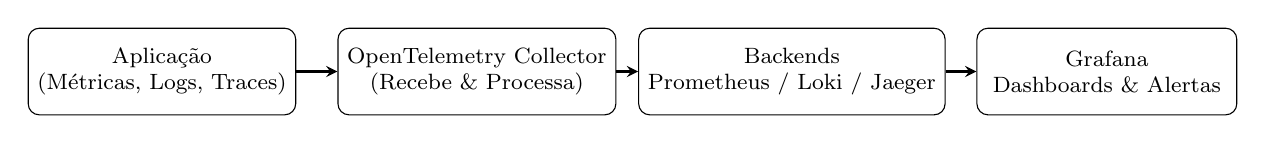
\begin{tikzpicture}[>=stealth,
    box/.style={rectangle,rounded corners,draw,minimum height=1.1cm,minimum width=3.3cm,align=center,font=\footnotesize}]
\node[box] (app) at (0,0) {Aplicação\\(Métricas, Logs, Traces)};
\node[box] (otel) at (4,0) {OpenTelemetry Collector\\(Recebe \& Processa)};
\node[box] (back) at (8,0) {Backends\\Prometheus / Loki / Jaeger};
\node[box] (graf) at (12,0) {Grafana\\Dashboards \& Alertas};
\draw[->,thick] (app)--(otel); \draw[->,thick] (otel)--(back); \draw[->,thick] (back)--(graf);
\end{tikzpicture}%
}
\caption{Pipeline simplificado de telemetria na arquitetura implementada}
\label{fig:pipeline_otel}
\end{figure}


\section{Detalhes Técnicos da Implementação}

\subsection{Estratégia de Instrumentação em .NET}

Do ponto de vista técnico, a instrumentação foi aplicada exclusivamente aos serviços criados internamente, evitando a recolha de dados de dependências externas. Desta forma, métricas, logs e traces refletem apenas o comportamento dos microsserviços proprietários, reduzindo o ruído e a sobrecarga de dados. Esta abordagem garante que a telemetria recolhida é relevante para a análise e otimização da plataforma R2UT, focando a monitorização nos elementos críticos sob responsabilidade direta da equipa de desenvolvimento.

A instrumentação de aplicações é um passo crucial para gerar dados de telemetria significativos. Em ambientes de microsserviços com múltiplas APIs, a instrumentação individual de cada serviço pode ser repetitiva e propensa a erros. Para mitigar esta complexidade, foi adotada uma abordagem prática e reutilizável para a instrumentação de APIs ASP.NET Core, utilizando um pacote comum (\textit{DTX.Base.Common}). Este pacote encapsula toda a configuração necessária para a emissão de \textit{traces} distribuídos, métricas e logs estruturados, promovendo uma padronização e um desacoplamento eficaz entre o código da aplicação e a infraestrutura de monitorização.

Esta estratégia centraliza a lógica de monitorização num único ponto, reduzindo significativamente o código repetido. A configuração da telemetria pode ser ativada e controlada dinamicamente através de variáveis de ambiente, conferindo flexibilidade e portabilidade entre diferentes ambientes (desenvolvimento, homologação e produção). Para instrumentar novos serviços, a intervenção necessária é mínima: basta adicionar o pacote \textit{DTX.Base.Common}, invocar um método de extensão no \texttt{Program.cs} e definir as variáveis de ambiente correspondentes.

A lógica de monitorização foi centralizada num único método de extensão, aplicado na inicialização de cada API \.NET:

\begin{verbatim}
builder.ConfigureOpenTelemetry();
\end{verbatim}

Este método ativa automaticamente os componentes do OpenTelemetry responsáveis pela instrumentação de \textit{tracing} distribuído, recolha de métricas e exportação de logs estruturados. As opções de configuração são controladas dinamicamente por variáveis de ambiente, evitando alterações no código ou recompilação ao migrar entre ambientes.


As variáveis de ambiente listadas na Tabela \ref{tab:otel_env_vars} são responsáveis por configurar a camada de exportação OTLP em cada microsserviço. Em vez de definir endpoints ou credenciais diretamente no código, estes parâmetros são injetados no ambiente de execução, permitindo separar configuração operacional da lógica de aplicação.

A variável \texttt{OTEL\_EXPORTER\_OTLP\_ENDPOINT} determina o endereço do Collector para onde os dados serão enviados, garantindo flexibilidade na migração entre ambientes (por exemplo, ambiente local, cluster de homologação ou produção em Kubernetes). A variável \texttt{OTEL\_EXPORTER\_OTLP\_PROTOCOL} define o protocolo de comunicação a utilizar, assegurando compatibilidade com diferentes configurações de rede e segurança. Por fim, \texttt{OTEL\_EXPORTER\_OTLP\_HEADERS} permite incluir cabeçalhos adicionais, como tokens de autenticação ou etiquetas de contexto, possibilitando uma integração segura e multi-tenant quando necessário.

Este modelo de configuração facilita a automação de \textit{deploys}, promove maior segurança operacional e reduz a necessidade de alterações no código ao longo do ciclo de vida do sistema.


\begin{table}[H]
\centering
\begin{tabular}{|p{6cm}|p{8cm}|}
\hline
\textbf{Variável} & \textbf{Descrição} \\ \hline
\texttt{OTEL\_EXPORTER\_OTLP\_ENDPOINT} & URL do \textit{endpoint} do Collector OTLP. \\ \hline
\texttt{OTEL\_EXPORTER\_OTLP\_PROTOCOL} & Protocolo utilizado (\textit{grpc} ou \textit{http/protobuf}). \\ \hline
\texttt{OTEL\_EXPORTER\_OTLP\_HEADERS} & Cabeçalhos opcionais no formato chave=valor (ex.: \texttt{Authorization=Bearer abc}). \\ \hline
\end{tabular}
\caption{Variáveis de ambiente utilizadas para configuração da exportação OTLP}
\label{tab:otel_env_vars}
\end{table}

Embora a instrumentação explícita via \texttt{DTX.Base.Common} fosse o padrão adotado, também foi avaliada a possibilidade de implementação da instrumentação \textit{zero-code} no ambiente .NET, utilizando agentes e configurações automáticas do \textit{OpenTelemetry}. No entanto, foram identificadas algumas limitações no controlo da granularidade dos dados e na integração com determinadas bibliotecas utilizadas internamente. Por esse motivo, optou-se por encapsular a instrumentação num pacote comum, garantindo padronização e flexibilidade.


\subsection{Vantagens da Abstração da Instrumentação OpenTelemetry}

O encapsulamento da lógica de instrumentação no pacote \texttt{DTX.Base.Common} e a exposição via um método de extensão (\texttt{ConfigureOpenTelemetry()}) proporcionam benefícios significativos para o desenvolvimento e a operação de aplicações distribuídas. De referir:

\begin{itemize}
\item \textbf{Padronização da Instrumentação entre Múltiplas APIs}, que garante que todas as APIs sigam as mesmas convenções de observabilidade, resultando em dados de telemetria consistentes e facilmente comparáveis. Isso é fundamental para a correlação eficaz de dados em sistemas complexos.

\item \textbf{Desacoplamento da Infraestrutura de Monitorização}, que faz com que o código da aplicação se torne independente das ferramentas de backend utilizadas (\textit{Grafana}, \textit{Jaeger}, \textit{Tempo}, etc.). Se houver uma mudança nas ferramentas de monitorização, as modificações são minimizadas e confinadas à configuração do Collector ou às variáveis de ambiente, não exigindo alterações no código da aplicação.

\item \textbf{Facilidade de Configuração via Ambiente}, que assegura que a ativação e o ajuste da observabilidade sejam feitos através de variáveis de ambiente, o que simplifica a implantação e a gestão em diferentes ambientes (desenvolvimento, homologação, produção), promovendo a portabilidade.

\item \textbf{Redução Significativa de Código Repetido}, que, ao centralizar a lógica de observabilidade num único ponto, evita a duplicação de código em cada novo serviço ou API, tornando o processo de instrumentação mais eficiente e menos propenso a erros.
\end{itemize}

Com esta abordagem, a instrumentação de novos serviços pode ser realizada com mínima intervenção, com a adição do pacote \texttt{DTX.Base.Common}, uma chamada simples ao método de extensão no \texttt{Program.cs} e a definição das variáveis de ambiente necessárias. Isso acelera o desenvolvimento e garante que a monitorização seja uma parte integrante do ciclo de vida da aplicação desde o início.


\section{Coleta de dados com o OpenTelemetry Collector}

A fase de coleta é o ponto de entrada para os dados de telemetria no pipeline de monitorização. É responsável por capturar logs, métricas e traces gerados pelas aplicações instrumentadas, agentes \textit{sidecar} ou ferramentas de terceiros. A coleta é feita principalmente através dos \textit{receivers} do \textit{OpenTelemetry Collector}, que atuam como ouvintes ou \textit{scrapers}, aceitando dados em vários formatos.

O \textit{OpenTelemetry Collector}, um componente central do ecossistema, funciona como um hub de processamento centralizado, capaz de lidar com múltiplas fontes e destinos de dados. Na implementação em questão, o Collector foi configurado para escutar em duas portas principais para o protocolo OTLP: \texttt{4317} para \texttt{gRPC} e \texttt{4318} para \texttt{HTTP}. Esta configuração permite que as aplicações enviem telemetria usando o protocolo de sua preferência. A fase de coleta é crítica, uma vez que é ela que garante que os dados cheguem de forma consistente e em tempo real ao pipeline de monitorização.

No ambiente \textit{Kubernetes}, a implantação do \textit{OpenTelemetry Collector} foi realizada como um \textit{DaemonSet}. Esta escolha de implantação garante que o Collector seja executado como um agente em cada nó (\textit{node}) do cluster, em vez de ser um serviço centralizado. Cada instância do \textit{DaemonSet Collector}, que age como um agente local, recebe a telemetria dos pods que estão no mesmo nó.

A principal vantagem desta abordagem é a redução de latência e a garantia de segurança. Ao coletar a telemetria localmente, os dados não precisam viajar pela rede do cluster, reduzindo a latência e o risco de congestionamento. Além disso, essa arquitetura de agente local é mais resiliente, pois a falha de um agente afeta apenas a coleta de dados de um único nó, enquanto os outros nós continuam a operar normalmente. Essa configuração de \textit{DaemonSet}, combinada com os \textit{receivers} do Collector, otimiza o fluxo de telemetria e torna-o mais robusto e eficiente.

\subsection{O Protocolo OTLP (gRPC/HTTP)}

O \textit{OpenTelemetry Protocol} (OTLP) é o protocolo padrão utilizado na plataforma de observabilidade para o transporte de dados de telemetria, como métricas, logs e \textit{tracing} distribuído. Desenvolvido como parte do ecossistema OpenTelemetry, o OTLP é um protocolo aberto, extensível e eficiente, que permite a comunicação entre aplicações instrumentadas, agentes de coleta como o \textit{OpenTelemetry Collector}, e sistemas de backend, como o \textit{Grafana Loki} (logs), o \textit{Jaeger} (traces) ou \textit{Prometheus} (métricas). O protocolo suporta os formatos \texttt{gRPC} e \texttt{HTTP/protobuf}, garantindo flexibilidade de integração com diversos ambientes e ferramentas. Num cluster Kubernetes, o uso do OTLP padroniza a coleta e exportação de dados de observabilidade entre os pods e os componentes da infraestrutura de monitorização, garantindo portabilidade, interoperabilidade e escalabilidade da solução implementada.

\subsection{OpenTelemetry Operator}

Gerir a observabilidade em ambientes Kubernetes pode tornar-se complexo, especialmente quando é necessário configurar múltiplos Collectors, manter consistência de \textit{pipelines} e aplicar boas práticas de escalabilidade e de segurança. Para simplificar esta gestão, a comunidade desenvolveu o \textit{OpenTelemetry Operator}, um \textit{Custom Kubernetes Operator} que automatiza o ciclo de vida dos Collectors e a sua configuração.

O \textit{OpenTelemetry Operator} expande o Kubernetes através de \textit{Custom Resource Definitions} (CRDs), introduzindo novos tipos de recurso que descrevem configurações de observabilidade de forma declarativa. O recurso mais importante é o \texttt{OpenTelemetryCollector}, no qual o utilizador define, em YAML, as características desejadas do Collector (\textit{receivers}, \textit{processors}, \textit{exporters} e modo de execução). O Operator traduz automaticamente essa especificação em objetos nativos do Kubernetes, como \textit{Deployments}, \textit{DaemonSets} ou \textit{ConfigMaps}. Dessa forma:

\begin{enumerate}
\item O programador ou DevOps aplica um manifesto \texttt{OpenTelemetryCollector};
\item O Operator valida e cria os recursos Kubernetes correspondentes;
\item O Collector é implantado de forma consistente e conforme as boas práticas definidas pela comunidade.
\end{enumerate}


O recurso \texttt{OpenTelemetryCollector}, disponibilizado pelo \textit{OpenTelemetry Operator}, permite definir, de forma declarativa, o modo de execução do Collector, conferindo elevada flexibilidade na adaptação da arquitetura de monitorização às características do sistema. Os principais modos de operação são:

\begin{itemize}
    \item \textbf{DaemonSet.} Executa uma instância do Collector em cada nó do cluster, recolhendo a telemetria localmente e reduzindo a latência e o tráfego de rede. Este modo é particularmente indicado para clusters de grande dimensão ou aplicações com elevado volume de métricas e logs.

    \item \textbf{Deployment.} Executa o Collector como um serviço centralizado, atuando como \textit{gateway} e agregando telemetria antes de a reenviar para os backends definidos. É uma opção recomendada para ambientes de desenvolvimento ou para arquiteturas onde a centralização seja operacionalmente vantajosa.

    \item \textbf{Sidecar.} Executa o Collector em conjunto com cada \textit{pod}, garantindo o nível máximo de isolamento e controlo sobre a instrumentação de cada serviço. Este modelo oferece monitorização altamente granular, embora com maior custo de recursos.

    \item \textbf{StatefulSet.} Utilizado em cenários onde é necessário garantir estado persistente ou uma configuração estável e ordenada, útil em pipelines de telemetria mais complexos ou ambientes de auditoria.
\end{itemize}

Além desta flexibilidade arquitetural, a utilização do \textit{OpenTelemetry Operator} oferece benefícios adicionais:


\begin{itemize}
    \item \textbf{Automação.} Elimina a necessidade de escrever e manter manualmente manifestos Kubernetes complexos para cada instância do Collector, simplificando significativamente a gestão operacional e reduzindo o risco de erros de configuração.

    \item \textbf{Consistência e padronização.} Garante que todas as instâncias do Collector são configuradas de forma homogénea e alinhadas com boas práticas, assegurando uniformidade na recolha e processamento da telemetria em todo o cluster.

    \item \textbf{Integração nativa com GitOps.} Por ser baseado em definições declarativas, integra-se facilmente com pipelines de CI/CD e ferramentas GitOps, como ArgoCD e Flux, facilitando a gestão versionada e auditável das configurações de monitorização.

    \item \textbf{Evolução contínua e alinhamento com a comunidade.} O Operator é mantido pela comunidade OpenTelemetry, garantindo compatibilidade com novas versões, boas práticas atualizadas e reduzindo o risco de configurações obsoletas ao longo do tempo.
\end{itemize}


Em síntese, o \textit{OpenTelemetry Operator} simplifica substancialmente a adoção de monitorização em Kubernetes, promovendo maior automação, padronização e escalabilidade, ao mesmo tempo que reduz o esforço manual e a probabilidade de erros operacionais.

\begin{figure}[H]
    \centering
    \includegraphics[width=0.8\textwidth]{images/Diagramas/daemonset_collector.png}
    \caption{Arquitetura de coleta local com \textit{OpenTelemetry Collector} em modo \textit{DaemonSet}.}
    \label{fig:otel-daemonset}
\end{figure}


A abordagem adotada neste trabalho foi a execução do \textit{OpenTelemetry Collector} como um \textbf{\textit{DaemonSet}}, disponibilizando um agente local em cada nó do cluster Kubernetes (Figura \ref{fig:otel-daemonset}). Em cada nó, um \textit{Pod} do Collector expõe \textit{receivers} OTLP por gRPC (porta 4317) e HTTP/Protobuf (porta 4318), recebendo métricas, logs e traces das \textit{workloads} residentes nesse nó.

Esta decisão foi guiada por três objetivos principais:

\begin{itemize}
    \item \textbf{Baixa latência na entrega de telemetria.} Evitando transmissões de rede adicionais antes do primeiro processamento;
    \item \textbf{Resiliência local.} Confinando o impacto de eventuais falhas ao nó específico, sem afetar o resto do cluster;
    \item \textbf{Simplicidade de integração.} Permitindo que as aplicações publiquem telemetria para um único \textit{endpoint} local, sem a necessidade de mecanismos adicionais de descoberta.
\end{itemize}

A adoção do padrão \textit{DaemonSet} resultou numa menor variabilidade na entrega dos sinais, com coleta e pré-processamento a nível local, isolamento de falhas por nó, redução da dependência de rede intra-cluster e uma configuração simplificada do lado das aplicações, uma vez que estas comunicam com um \textit{endpoint} local único.


\section{Processamento e Transformação dos Dados}

Após a sua recolha, os dados de telemetria passam por uma fase crítica de processamento dentro do \textit{OpenTelemetry Collector}. Esta etapa, orquestrada por diversos \textit{processors}, é essencial para modificar, enriquecer, agrupar ou filtrar os dados, assegurando a sua consistência, eficiência e utilidade para os sistemas subsequentes de armazenamento e análise.


\subsection{Processadores e as suas Aplicações}

Após a fase de recolha, os dados de telemetria passam por um estágio fundamental de processamento dentro do \textit{OpenTelemetry Collector}. Este processamento é realizado por um conjunto de \textit{processors}, responsáveis por transformar, enriquecer, agrupar e filtrar os dados. Esta etapa assegura que a telemetria seja consistente, eficiente e alinhada com as necessidades de análise, conformidade e desempenho da solução implementada.

De forma a consolidar o papel de cada componente, a Tabela \ref{tab:otel-processors} apresenta os principais \textit{processors} utilizados, a sua função primária e respetivas aplicações práticas.

\begin{table}[H]
\centering
\caption{Principais \textit{processors} do OpenTelemetry Collector utilizados}
\label{tab:otel-processors}
\begin{tabular}{|p{3cm}|p{4cm}|p{4.2cm}|p{4.2cm}|}
\hline
\textbf{Processor} & \textbf{Função Primária} & \textbf{Aplicações Chave} & \textbf{Benefício para Monitorização} \\ \hline
\texttt{transform} & Modifica dados com OTTL. & Adiciona \texttt{service.name}, normaliza severidade, converte timestamps. & Consistência semântica e refinamento da telemetria. \\ \hline
\texttt{batch} & Agrupa dados em lotes. & Reduz chamadas de rede e overhead. & Melhora o débito e otimiza a exportação. \\ \hline
\texttt{attributes} & Adiciona ou altera atributos. & Injeta metadados como ambiente e host. & Melhora correlação, filtragem e contexto. \\ \hline
\texttt{resource} & Modifica atributos de recurso. & Garante aplicação uniforme de \texttt{service.name}, versão, ambiente. & Uniformidade e correta identificação de origem dos dados. \\ \hline
\texttt{memory\_limiter} & Controla consumo de memória. & Evita saturação e falha do Collector. & Estabilidade operacional. \\ \hline
\texttt{tail\_sampling} & Amostragem com base no trace completo. & Seleciona traces críticos (ex.: erros, alta latência). & Reduz volume e custo mantendo visibilidade de incidentes. \\ \hline
\end{tabular}
\end{table}

\begin{itemize}
% [label=\textbf{\arabic*.}, leftmargin=1.2cm]

\item \textbf{Processador \texttt{transform}}\\
% \subsubsection{Processador \texttt{transform}}

O processador \texttt{transform} utiliza a \textit{OpenTelemetry Transformation Language} (OTTL) para realizar modificações avançadas nos dados de telemetria. Na implementação atual, é utilizado para adicionar o atributo \texttt{service.name} aos sinais de telemetria, converter \textit{timestamps} para um formato padronizado, normalizar níveis de severidade de logs (por exemplo, mapeando diferentes níveis para categorias consistentes como \texttt{INFO}, \texttt{WARN} e \texttt{ERROR}), e aplicar regras de amostragem dinâmica a \textit{traces}. No entanto, devido ao seu elevado grau de flexibilidade e poder expressivo, a sua configuração deve ser cuidadosamente validada para evitar \textit{transformações inconsistentes} (\textit{Unsound Transformations}) ou \textit{conflitos de identidade} (\textit{Identity Conflicts}), que podem comprometer a integridade e a fiabilidade da telemetria.

\clearpage

\item \textbf{Processador \texttt{batch}}\\
% \subsubsection{Processador \texttt{batch}}

Este processador agrupa eficientemente os dados de telemetria em lotes antes de serem exportados. O batching reduz significativamente o número de chamadas de rede e a sobrecarga associada, melhorando assim o débito geral e a eficiência da exportação de dados, especialmente em ambientes de alto volume

\item \textbf{Processador \texttt{attributes}}\\
% \subsubsection{Processador \texttt{attributes}}

O processador \texttt{attributes} permite adicionar, modificar ou remover atributos (metadados) associados a \textit{spans}, logs ou métricas. Na prática, este processador é utilizado para enriquecer os dados de telemetria com informação contextual relevante - por exemplo, injetando um atributo estático que identifica o ambiente de execução (como \textit{produção} ou \textit{desenvolvimento}) ou acrescentando metadados ao nível do \textit{host}. Este enriquecimento é fundamental para consultas mais eficientes, filtragem precisa e correlação robusta entre diferentes sinais, contribuindo para uma análise mais clara e completa do comportamento do sistema distribuído.

\item \textbf{Processador \texttt{resource}}\\
% \subsubsection{Processador \texttt{resource}}


Este processador tem como objetivo a modificação de atributos de recurso, os quais descrevem a entidade responsável pela geração da telemetria, como o serviço da aplicação, a máquina \textit{host} ou o \textit{container}. É essencial para anexar de forma consistente metadados fundamentais, tais como \textit{environment}, \textit{service version} ou \textit{region} às métricas e para enriquecer logs com informação contextual detalhada. O processador \texttt{resource} assegura que atributos de identificação comuns, nomeadamente \texttt{service.name}, são aplicados uniformemente a todos os sinais de telemetria (logs, \textit{traces} e métricas). Esta consistência é crucial para permitir uma correlação eficiente e precisa entre sinais no Grafana.

\item \textbf{Processador \texttt{memory\_limiter}}\\
% \subsubsection{Processador \texttt{memory\_limiter}}

Este processador é utilizado para evitar que o OpenTelemetry Collector consuma uma quantidade excessiva de memória. Ao definir limites explícitos de utilização, previne que o processo do Collector falhe devido ao esgotamento de recursos, garantindo assim a estabilidade e a fiabilidade contínuas de todo o \textit{pipeline} de monitorização. Esta salvaguarda é especialmente importante em ambientes de elevada carga, onde picos de telemetria podem ocorrer de forma imprevisível.


\item \textbf{Processador \texttt{tail\_sampling}}\\
% \paragraph{Processador \texttt{tail\_sampling}.}

Este processador permite tomar decisões de amostragem com base no contexto completo de um \textit{trace}, ou seja, apenas após todos os \textit{spans} associados terem sido recebidos. Suporta múltiplos critérios de filtragem que podem ser combinados, incluindo amostragem baseada na latência observada, taxas probabilísticas, códigos de estado HTTP (por exemplo, apenas \textit{traces} com erro) ou limites de taxa. 

Esta abordagem de amostragem baseada no contexto completo do trace é fundamental para controlar o volume de dados gerados por sistemas distribuídos de elevado tráfego, permitindo reter apenas os \textit{traces} mais relevantes para diagnóstico e análise. O seu uso contribui para otimizar custos de armazenamento e melhorar o desempenho de consultas no \textit{backend} de \textit{tracing}, mantendo a capacidade de capturar e investigar \textit{traces} críticos ou anómalos.

\end{itemize}

A capacidade do \textit{OpenTelemetry Collector} de modificar todos os aspetos da telemetria, incluindo a remoção de informações sensíveis através do processador \texttt{transform} ou o enriquecimento consistente de dados com atributos específicos, posiciona-o como um ponto de controlo estratégico na governação de dados. Esta centralização do controlo significa que os requisitos de conformidade podem ser geridos e aplicados ao nível do Collector, reduzindo a necessidade de alterações individuais nas aplicações ou de configurações complexas específicas dos \textit{backends}.

Esta abordagem não só centraliza significativamente o controlo de dados, como também minimiza a superfície de ataque para fugas acidentais de informação. Além disso, a capacidade de filtrar, agrupar e reduzir a cardinalidade dos dados antes da sua exportação para os \textit{backends} traduz-se diretamente em poupanças substanciais nos custos de ingestão e armazenamento, especialmente em serviços de observabilidade geridos. Ao reduzir o volume e a complexidade dos dados na origem, o Collector melhora o desempenho das consultas nos \textit{backends} e mitiga potenciais problemas de ``crise de identidade'' em métricas, resultando em \textit{dashboards} mais fiáveis. Assim, o Collector assume-se como um componente crítico para assegurar tanto a eficiência económica como a eficiência operacional de toda a \textit{stack} de monitorização.



\section{Persistência e Armazenamento de Dados }

A seleção dos sistemas de \textit{backend} para armazenar \textit{logs}, \textit{traces} e métricas foi realizada de acordo com os requisitos definidos pela empresa, que recomendou soluções maduras e amplamente adotadas no ecossistema de monitorização. Estas ferramentas foram utilizadas exclusivamente como \textit{backends}, tendo como principal objetivo centralizar o armazenamento e a análise dos dados exportados pelos microsserviços, sem adicionar dependências diretas ao código das aplicações.

\subsection{Armazenamento de \textit{Logs} com o Loki}
O Loki foi escolhido como sistema de armazenamento de \textit{logs} devido à sua arquitetura otimizada para consultas baseadas em etiquetas (\textit{labels}), em vez de pesquisa textual completa (\textit{full-text search}). Esta abordagem torna-o mais eficiente e menos dispendioso em termos de recursos quando comparado com soluções tradicionais, como o Elasticsearch. 

Os \textit{logs} estruturados emitidos pelas APIs .NET são enviados ao \textit{OpenTelemetry Collector} através do protocolo OTLP e, posteriormente, exportados para o Loki. A integração nativa com o Grafana permite que os \textit{logs} sejam visualizados e correlacionados com métricas e \textit{traces}, proporcionando uma análise centralizada e coerente do sistema.

\subsection{Armazenamento de \textit{Traces} com o Jaeger}
O Jaeger foi adotado como \textit{backend} de armazenamento e análise de \textit{traces} distribuídos, dada a sua capacidade comprovada de fornecer visibilidade \textit{end-to-end} sobre o ciclo de vida de uma requisição. Com base no atributo \texttt{service.name}, é possível segmentar e filtrar os \textit{traces}, identificando gargalos e potenciais pontos de falha durante a interação entre microsserviços.

Os dados são exportados pelo \textit{OpenTelemetry Collector} via OTLP/\textit{gRPC} para o \textit{endpoint} do Jaeger, onde ficam persistidos para consulta e inspeção detalhada, sendo posteriormente visualizados através do Grafana.

\subsection{Armazenamento de Métricas com o Prometheus}
O Prometheus foi selecionado como sistema de armazenamento de métricas devido à sua robustez no processamento de séries temporais e à linguagem de consulta PromQL, que possibilita análises avançadas e precisas. As métricas das aplicações .NET são recolhidas pelo \textit{OpenTelemetry Collector} e exportadas para o Prometheus, evitando exposição direta dos serviços e centralizando a captura de telemetria.

Complementarmente, as métricas de infraestrutura provenientes do \textit{Node Exporter} são recolhidas diretamente pelo Prometheus através de \textit{scraping} HTTP. Esta abordagem combinada assegura visibilidade tanto ao nível da aplicação como da infraestrutura, proporcionando uma visão abrangente e consistente do desempenho do sistema.

\chapter{Visualização e Análise de Dados}

\section{Visualização centralizada no Grafana}

A visualização dos dados de telemetria assume um papel crucial para a compreensão e monitorização eficaz de sistemas distribuídos. Embora as ferramentas Prometheus, Jaeger e Loki disponham de interfaces próprias para análise independente de métricas, traces e logs, a fragmentação das informações pode dificultar a correlação rápida entre estes dados. Por esse motivo, optou-se pelo Grafana como camada de visualização unificada, visando uma experiência integrada e eficiente.

Entre as principais vantagens destacam-se:

\begin{itemize}
    \item Centralização das métricas, logs e traces num único painel interativo;
    \item Capacidade avançada de correlação entre diferentes tipos de dados, facilitando a identificação de causas-raiz nas anomalias;
    \item Configuração unificada de alertas que abrange todas as fontes de dados;
    \item Interface intuitiva e personalizável, acessível para diversos perfis técnicos;
    \item Linguagens de consulta especializadas (PromQL, LogQL) diretamente integradas.
\end{itemize}

Assim, o Grafana habilita uma abordagem de "single pane of glass", essencial para o acompanhamento consolidado do desempenho e saúde do sistema e traces de chamadas entre serviços, com visualização temporal.

\break

\section{Organização dos Dashboards}

Os dashboards no Grafana foram estruturados em três categorias principais:

\begin{itemize}
    \item \textbf{Métricas da Aplicação}: monitorização do número de requisições HTTP por segundo, latência média e percentis (p95 e p99), taxas de erro 4xx e 5xx, além do uso de memória da aplicação \texttt{.NET};
    \item \textbf{Infraestrutura Kubernetes}: dados provenientes do Node Exporter relativos à utilização de CPU por nó e pod, carga do sistema (load average), e espaço de disco e memória física utilizados;
    \item \textbf{Logs e Traces}: visualização de logs estruturados filtrados por nível, mensagem e nome do serviço, análise de spans por rota, duração e código de estado, bem como visualização temporal das chamadas entre serviços através dos traces.
\end{itemize}

Esta organização aprimora a navegação e facilita a análise rápida e contextualizada.

\subsection{Paineis e Dashboards}

Para efeito de apresentação e análise, os dashboards apresentados neste capítulo focam-se exclusivamente nos dados relativos ao serviço específico TicketsManagement. Embora fosse perfeitamente possível incluir visualizações de outros ser-viços da arquitetura, tal abordagem tenderia a revelar informações redundantes, uma vez que os padrões e métricas observados seriam semelhantemente aplicáveis. Assim, esta escolha visa proporcionar uma análise mais clara e exemplar, evitando a dispersão do foco e privilegiando a profundidade sobre a generalidade.

\begin{figure}[H]
    \centering
    \includegraphics[width=1\textwidth]{images/Grafana/all_logs_dashboard.png}
    \caption{Painel global de Logs}
    % \label{fig:digital_twin}
\end{figure}

\begin{figure}[H]
    \centering
    \includegraphics[width=1\textwidth]{images/Grafana/error_logs_dashboard.png}
    \caption{Painel de Logs de Erro}
    % \label{fig:digital_twin}
\end{figure}

\begin{figure}[H]
    \centering
    \includegraphics[width=1\textwidth]{images/Grafana/dashboard.png}
    \caption{\textit{Dashboard} de \textit{Logs}}
    % \label{fig:digital_twin}
\end{figure}

\begin{figure}[H]
    \centering
    \includegraphics[width=1\textwidth]{images/Grafana/cpu_memory_dashboard.png}
    \caption{Uso de CPU e Memória}
    % \label{fig:digital_twin}
\end{figure}

\begin{figure}[H]
    \centering
    \includegraphics[width=1\textwidth]{images/Grafana/metrics_dashboard.png}
    \caption{Dashboard de metricas: p95, Taxa de Erro, Pedidos por segundo}
    % \label{fig:digital_twin}
\end{figure}

\section{Correlação entre Logs e Traces}

Um dos principais ganhos trazidos pelo Grafana é a correlação direta entre logs e traces. Com um dashboard dedicado, foi possível implementar múltiplos filtros, incluindo o \texttt{service\_name}, que permitem visualizar os logs emitidos por diferentes serviços e vinculá-los diretamente às requisições (traces) correspondentes que os originaram.

Cada entrada de log disponibiliza um link direto para o trace associado, simplificando significativamente a depuração e o diagnóstico de problemas. Este recurso proporciona uma visão holística do estado do sistema e das suas interações, facilitando a identificação rápida de causas de falhas ou degradação do serviço.

\begin{figure}[H]
    \centering
    \includegraphics[width=1\textwidth]{images/Grafana/log_expanded.png}
    \caption{Log: Correlação Log e Trace}
    % \label{fig:digital_twin}
\end{figure}

\begin{figure}[H]
    \centering
    \includegraphics[width=1\textwidth]{images/Grafana/trace link por log.png}
    \caption{Link para Trace}
    % \label{fig:digital_twin}
\end{figure}

\begin{figure}[h]
    \centering
    \includegraphics[width=1\textwidth]{images/Grafana/trace_approve.png}
    \caption{Trace: Correlação Log e Trace}
    % \label{fig:digital_twin}
\end{figure}

\section{Alertas}

todo: falar um pouco sobre os alertas, ainda nao implementados, mas de configuracao muito simples
\chapter{Conclusões e Trabalho Futuro}

\section{Conclusões}

O trabalho desenvolvido permitiu conceber e implementar uma solução de monitorização e observabilidade para o projeto \textit{R2UT}, reforçando a visibilidade e a resiliência da sua infraestrutura de microserviços. A integração das ferramentas \textit{open source} \textit{Prometheus}, \textit{Grafana}, \textit{Loki}, \textit{Jaeger} e \textit{OpenTelemetry Collector} revelou-se eficaz para recolher, centralizar e correlacionar métricas, \textit{logs} e \textit{traces} de forma padronizada.

Durante o desenvolvimento, foram superados diversos desafios técnicos relacionados com a orquestração dos componentes, a instrumentação da aplicação e a gestão de recursos em ambiente \textit{cloud-native}. Estes obstáculos contribuíram para um melhor entendimento das boas práticas de observabilidade e consolidaram a robustez da solução final.  

Os resultados obtidos demonstram uma redução significativa dos tempos médios de deteção e resolução de incidentes (\textit{MTTD} e \textit{MTTR}), bem como uma melhoria da estabilidade operacional do sistema. Em síntese, foi validada a viabilidade de uma pilha de observabilidade escalável e aberta, totalmente baseada em tecnologias de utilização livre, alinhada com os objetivos do projeto \textit{R2UT}.

\section{Trabalho Futuro}

Como continuidade deste trabalho, prevê-se a expansão da solução de observabilidade através da integração de mecanismos de automação e inteligência artificial para análise preditiva de métricas e deteção de anomalias. A aplicação de técnicas de \textit{machine learning} poderá permitir a antecipação de falhas e a geração de alertas inteligentes com base em padrões históricos de comportamento.

Adicionalmente, pretende-se aprofundar a integração com ferramentas de orquestração em larga escala, avaliando o desempenho do sistema em ambientes \textit{multi-tenant} e cenários de elevada carga. Também se prevê a criação de painéis avançados de \textit{dashboards} e relatórios dinâmicos, bem como o estudo de políticas de \textit{autoscaling} e de recuperação automática de serviços.

Por fim, a disseminação dos resultados e a integração desta solução no ecossistema de produção da plataforma \textit{R2UT} representam uma oportunidade de validação real do seu impacto, contribuindo para uma infraestrutura mais inteligente, resiliente e observável.


\renewcommand{\baselinestretch}{1}
\bibliographystyle{plainnat}
\bibliography{dissertation}
\printindex

% \appendix
% \renewcommand\chaptername{Apêndice}

% \part{Apêndices}

% \input{appendices/SupportWork}
% \chapter{Details of results}

\section{Example JSON body for creation of device via API}
\label{appendix:example}
\begin{verbatim}
  {
  "policyId": "org.eclipse ditto:577247a5-1438-48d5-b485-d41f673cac61",
  "definition": "com.smarttech:thermostat:1.0.0",
  "attributes": {
    "manufacturer": "SmartTech Solutions",
    "location": "New York, Office 2A",
    "serialno": "T10039284",
    "model": "ThermoX Pro 2000"
  },
  "features": {
    "temperature-control": {
      "definition": [
        "com.smarttech:thermostat:1.0.0"
      ],
      "properties": {
        "currentTemperature": 22.5,
        "targetTemperature": 24,
        "mode": "heating"
      }
    },
    "humidity-sensor": {
      "properties": {
        "configuration": {
          "samplingRateSeconds": 60,
          "thresholdAlert": 70
        },
        "status": {
          "humidityLevel": 45,
          "lastUpdated": "2025-06-24T10:00:00Z"
        }
      }
    }
  }
}
\end{verbatim}

\section{Thermostat DBIRTH payload in MQTT}
\label{appendix:details-of-resultsdbirth}
\begin{verbatim}
{
  "timestamp": {
    "low": -1719890226,
    "high": 408,
    "unsigned": true
  },
  "metrics": [
    {
      "name": "Temperature",
      "alias": {
        "low": 1,
        "high": 0,
        "unsigned": true
      },
      "timestamp": {
        "low": -1719890226,
        "high": 408,
        "unsigned": true
      },
      "datatype": 10,
      "isNull": true,
      "properties": {
        "keys": [
          "engUnits",
          "permission"
        ],
        "values": [
          {
            "type": 12,
            "stringValue": "inHg"
          },
          {
            "type": 12,
            "stringValue": "read-write"
          }
        ]
      }
    },
    {
      "name": "Device Control/Rebirth",
      "alias": {
        "low": 2,
        "high": 0,
        "unsigned": true
      },
      "timestamp": {
        "low": -1719890226,
        "high": 408,
        "unsigned": true
      },
      "datatype": 11,
      "isNull": true,
      "properties": {
        "keys": [
          "engUnits",
          "permission"
        ],
        "values": [
          {
            "type": 12,
            "stringValue": "inHg"
          },
          {
            "type": 12,
            "stringValue": "read-write"
          }
        ]
      }
    }
  ],
  "seq": {
    "low": 14,
    "high": 0,
    "unsigned": true
  }
}
\end{verbatim}

\section{Thermostat payload in MQTT for DDATA}
\label{appendix:details-of-resultsddata}
\begin{verbatim}
{
  "timestamp": {
    "low": -1719847593,
    "high": 408,
    "unsigned": true
  },
  "metrics": [
    {
      "alias": {
        "low": 1,
        "high": 0,
        "unsigned": true
      },
      "timestamp": {
        "low": -1719847593,
        "high": 408,
        "unsigned": true
      },
      "datatype": 10,
      "properties": {
        "keys": [
          "engUnits"
        ],
        "values": [
          {
            "type": 12,
            "stringValue": "inHg"
          }
        ]
      },
      "doubleValue": 3.2944017837137736
    },
    {
      "alias": {
        "low": 2,
        "high": 0,
        "unsigned": true
      },
      "timestamp": {
        "low": -1719847593,
        "high": 408,
        "unsigned": true
      },
      "datatype": 11,
      "properties": {
        "keys": [
          "engUnits"
        ],
        "values": [
          {
            "type": 12,
            "stringValue": "inHg"
          }
        ]
      },
      "booleanValue": false
    }
  ],
  "seq": {
    "low": 15,
    "high": 0,
    "unsigned": true
  }
}
\end{verbatim}

% \input{appendices/Listings}
% \input{appendices/Tooling}

\input{covers/BackCover}

\end{document}
